\documentclass[a4paper, 11pt]{report} %twoside
\title{Invproy\space $\alpha$}
\author{David Davó Laviña}
\date{\today{}}

%%Packages
\usepackage[utf8]{inputenc} %Para saber el encoding del archivo
\usepackage[T1]{fontenc}
%\usepackage[no-math]{fontspec} %Para usar fuentes del sistema
\usepackage{fontspec}

\usepackage{inconsolata}
\usepackage{uarial}

\usepackage[xindy, nomain, acronym, acronyms, nonumberlist, nopostdot, toc]{glossaries}
\usepackage{glossary-mcols}
%\usepackage{glossary-custom}

\usepackage[ampersand]{easylist} %Cosas de listas

\usepackage{titlesec}

\usepackage{graphicx} %Para insertar gráficos
\usepackage{float} %PAra posicionar bien los gráficos
\usepackage{unicode-math} %Para símbolos matemagicos
\usepackage[type={CC}, modifier={by-sa}, version={4.0}]{doclicense} %Muestra la licencia
\usepackage[usenames,svgnames,table]{xcolor} %Para darle color
\usepackage{dirtytalk} %Usado para citar
\usepackage{fvextra}
\usepackage{csquotes} %lo mismo que el anterior pero con estilo
\usepackage[spanish]{babel} %Hace que el idioma de los defaults esté en Español
\usepackage{fancyhdr} %Para poner encabezados y pies de página
%De la bibliografía y las citas.
\usepackage[
backend=biber,
style=ieee
]{biblatex}

\addbibresource{Bibl.bib}
	
\titleformat{\chapter}[display]
    {\color{Black}\normalfont\huge\bfseries}
    {\color{Black}\chaptertitlename\ \thechapter}{20pt}{\Huge}
\titlespacing*{\chapter}{0pt}{-10pt}{10pt}

%\chapterfont{\color{DarkRed}}
%\sectionfont{\color{FireBrick}}

%Decoraciones y formato del texto
\usepackage[left=3cm, right=3cm, top=3cm, bottom=3cm]{geometry}

\usepackage[cache=false]{minted} %Para insertar código

\usepackage{tabularx} %Para hacer tablas muy bonicas
\usepackage{multirow}
\usepackage{array}

\usepackage{caption}%Para insertar cosillas
\usepackage{subcaption}
\usepackage{sidecap}

\usepackage[normalem]{ulem}

\setmainfont{Arial}
\setmonofont{Inconsolata}

\setmathrm{Asana-Math.otf}
\setmathsf{Arial}
\setmathtt{Inconsolata}

\fontsize{11}{14}
%Pies de pagina y eso
\pagestyle{fancy}
\fancyhf{}
\makeatletter
\fancyhead[LE, RO]{\@author}
\fancyhead[RE, LO]{\@title}
\fancyfoot[LE, RO]{\thepage}
\fancyfoot[C]{\leftmark}

\makeglossaries
\newglossaryentry{Libr}
{
	name=Librería,
	description={En informática, una librería o biblioteca es un conjunto de recursos y fucniones diseñadas para ser usadas por otros programas. Incluyen plantillas, funciones y clases, subrutinas, código escrito, variables predefinidas...},
	plural=librerías,
}
\newglossaryentry{datos}{
	name=Datos,
	description={Secuencia binaria de unos y ceros que contiene información codificada},
	plural=Datos, 
}
\newacronym{gnu}{GNU}{\textit{GNU's Not Unix} (GNU no es Unix)}
\newglossaryentry{Linux}
{
  name=Linux,
  description={is a generic term referring to the family of Unix-like
               computer operating systems that use the Linux kernel},
  plural=Linuces
}
\newglossaryentry{conmutacion de paquetes}{
	name={Conmutación de paquetes},
	description={Método para enviar datos por una red de computadoras. Se divide el paquete en dos partes, una con información de control que leen los nodos para enviar el paquete a su destino y los datos a enviar},
}
\newacronym{osi}{OSI}{\textit{Open Systems Interconnection} (Interconexión de Sistemas Abiertos)}
\newglossaryentry{gls-ISO}{
	name={\textit{International Organization for Standardization}},
	description={Organización Internacional de Normalización. Compuesta de varias organizaciones nacionales se encarga de la creación de estándares internacionales desde 1947.},
}
\newacronym[see={[Glossary:]{gls-ISO}}]{iso}{ISO}{\textit{International Organization for Standardization}\glsadd{gls-ISO}}
\newglossaryentry{capas de abstraccion}{
	name={capas de abstracción},
	description={Método de ocultar detalles de implementación de un set de funcionalidades},
}
\newacronym{IEEE}{IEEE}{Instituto de Ingeniería Eléctrica y Electrónica}
\newglossaryentry{topologia de red}{
	name={topología de red},
	description={Configuración espacial o física de la red. (Ver \ref{topdred} pág.\pageref{topdred})},
	plural={topologías de red},
	see={topologia}
}
\newglossaryentry{topologia}{
	name={topología},
	description={``Rama de las matemáticas que trata especialmente de la continuidad y de otros conceptos más generales originados de ella, como las propiedades de las figuras con independencia de su tamaño o forma." \cite{rae}[Topología]},
	plural={topologías},
}
\newglossaryentry{hardware}{
	name={hardware},
	description={Conjunto de elementos físicos o materiales que constituyen un sistema informático.},
}
\newacronym{MAC}{MAC}{\textit{Media Access Control}, Control de Acceso al Medio}
\newacronym{ADSL}{ADSL}{\textit{Asymmetric Digital Subscriber Line} [Línea de Abonado Digital Asimétrica]}
\newacronym{LAN}{LAN}{\textit{Local Area Network} [Red de Área Local]}
\newacronym{FTTH}{FTTH}{\textit{Fiber To The Home} [Fibra hasta el hogar]}
\newacronym[see={[Glossary:]{gls-FTTx}}]{FTTx}{FTTx}{\textit{Fiber to the X \glsadd{gls-FTTx}}}
\newglossaryentry{gls-FTTx}{
	name={FTTx},
	description={Término que agrupa las distintas configuraciones de acometida de la fibra óptica.},
}
\newglossaryentry{bit}{
	name={bit},
	description={\textit{\textbf{Bi}nary digi\textbf{t}, o dígito binario. Cada dígito del sistema de numeración binario}},
	plural={bits}
}
\newacronym{POP3}{POP3}{\textit{Post Office Protocol}, Protocolo de Oficina Postal}
\newacronym{url}{URL}{\textit{Uniform Resource Identifier}, Identificador de Recursos Uniforme}
\newglossaryentry{cache}{
	name={caché},
	description={Almacenamiento temporal de datos con el objetivo de reducir el retardo, la carga de los servidores y el ancho de banda consumido},
}
\newglossaryentry{programacion imperativa}{
	name={programación imperativa},
	description={Las órdenes del programa cambian el estado de este mismo. Por ejemplo, una variable no tiene por que ser declarada con antelación y su valor es modificable. Es la que usa el código máquina de los ordenadores},
}
\newglossaryentry{botnet}{
	name={botnet},
	description={Grupo de ordenadores coordinados conectados a un maestro mediante un virus. Gracias a este virus se pueden realizar tareas masivas como el envío de SPAM o ataques DDoS},
}
\newglossaryentry{bug}{
	name={bug},
	plural={bugs},
	description={Error en un programa informático.},
}
\newglossaryentry{repositorio}{
	name={repositorio},
	plural={repositorios},
	description={Servidor donde se alojan ficheros o archivos para su descarga},
}
\newglossaryentry{dependencia}{
	plural={dependencias},
	name={dependencia},
	description={De un programa, otro tipo de software necesario para que éste funcione}
}
\newacronym{FSF}{FSF}{\textit{Free Software Foundation}, Fundación del Software Libre}
\newacronym{IDE}{IDE}{Entorno de Desarrollo Integrado, \textit{Integrated Development Enviroment}}
\newacronym{GUI}{GUI}{Interfaz Gráfica de Usuario, \textit{Graphic User Interface})}

%%% Algunas macros
\newcommand{\acr}[1]{\acrshort{#1} (\acrlong{#1})}
\DeclareFontShape{EU1}{Inconsolata(0)}{bx}{n}{<->ssub*Inconsolata(0)/m/n}{}
\usepackage{setspace}
%\onehalfspacing
%\linespread{1.25}
\linespread{1.5}

%Document
\begin{document} %#######################

\makeatletter
\begin{titlepage}
\centering
\vspace*{4cm}
{\scshape\LARGE IES Palas Atenea \par}
\vspace{1cm}
{\scshape\Large Proyecto de Investigación Bachillerato de excelencia:\\
Programación, redes y software libre\par}
\vspace{1.5cm}
{\fontsize{35pt}{40pt}\bfseries\color{DarkRed} \@title\par}
{\huge\bfseries Un simulador de redes por y para alumnos \par}
\rule{0.5\textwidth}{1pt}\par
\vspace{2cm}
{\Large\itshape \@author\par}
\vfill
Tutor\par
Julio Sánchez Olías

\vfill

{\large \@date\par}
\pagenumbering{gobble}
\end{titlepage}
\clearpage
\pagenumbering{Roman}

\tableofcontents
\listoffigures[Todas las imágenes son de autoría propia.]
\newpage{}
\setlength{\parskip}{5pt plus4pt minus3pt}

\chapter*{Introducción}
\addcontentsline{toc}{chapter}{Introducción}
En el mundo contemporáneo, ninguna de las innovaciones tecnológicas sería posible sin algo fundamental: las redes; y, más concretamente, redes informáticas. Las redes informáticas han hecho posible, desde su nacimiento, la comunicación de grandes sumas de datos a velocidades casi instantáneas entre sitios distantes. Al principio esta tecnología era usada entre universidades, acelerando el proceso de investigación al coordenarse unas universidades con otras mucho más rápidamente. 

Más tarde, se extendió el uso de esta tecnología del uso militar y científico a todas las empresas y hogares, comenzando así una revolución tecnológica que aún no se ha conseguido parar. Con acceso instantáneo a cultura, entretenimiento, conocimiento, información y más de dos mil exabytes de ancho de banda\footnote{Datos a Mayo de 2015. Fuente: Cisco--\cite{Cisco}} viajando por la red, se ha convertido en una herramienta de uso por la humanidad imprescindible para cualquier actividad.

Esto tampoco habría sido posible, en parte, gracias al software libre y al desarrollo colaborativo, ya que ha permitido el desarrollo de sistemas operativos como GNU/Linux de la \textit{Free Software Foundation} (Usado actualmente por el 90\% de los servidores de red) o CUPS (Creado por \textit{Apple Inc.}), el software para servidores de administración de impresoras más completo y competente usado en la mayoría de oficinas.

Son dos cosas muy importantes, que apenas son enseñadas en las clases de la ESO y Bachillerato, por eso he creado InvProy, un pequeño simulador de redes con la ambición de enseñar tanto de redes como de programación. Podrán experimentar, de una forma sencilla y muy visual como funciona una red y cómo se comportan los distintos protocolos. También, al ser software libre, los alumnos podrán aprender sobre programación al observar el código y tener la licencia para modificarlo y colaborar en el desarrollo del programa. Aunque el programa este aún en fase Alpha (fase de desarrollo), ya tiene la base para que sea muy sencillo añadir más protocolos, funcionalidades o dispositivos de red. A día de hoy tiene como dispositivos los ordenadores, conmutadores y concentradores. En cuanto a paquetes de red, permite enviar un Ping, usando los protocolos ICMP, IPv4 y Ethernet. 

\renewcommand{\abstractname}{Abstract}
\addcontentsline{toc}{section}{Abstract}
\begin{abstract}
There is a lot of software with the sole purpose of learning, but almost all of it is propietary software, and is also created by professionals; but there is some software with which students can learn how to code: software libre. Learning is even better if it is created by enthusiastic learners, because the code is easier to read by non-professionals and enthusiasts.\\
That is why we created \textit{InvProy} a Software Libre network simulation program (still in Alpha version) that contains more than four thousand lines of source code. Designed with learning and teaching purposes, both on networking and programming, it is written in the Python programming language and uses the Gtk+ library for the Graphics User Interface. At the moment it supports sending Ping’s while using the IEEE 802.11, TCP/IP and ICMP protocols. But as it is software libre, everybody can contribute to it so it will become a more complete program soon, in terms of functionalities and usability.
\end{abstract}

\chapter*{Agradecimientos}
Lo primero, me gustaría agradecer a mi familia; sobre todo a mis padres, \textbf{Anselmo y Gloria}, por aguantarme durante los meses de creación de este proyecto; y a mi tía, \textbf{Toñi}, por ayudarme a corregir poco a poco todas las impurezas del proyecto.

Quiero agradecer también a mis antiguos profesores del \textbf{IES Miguel Delibes} ya que, sin ellos, sí que no habría sido posible la realización de este trabajo ya que no estaría en este programa de bachillerato. Gracias \textbf{David Miguel}, \textbf{Alicia Valiente}, \textbf{Óscar Pintado}, \textbf{Raúl Castellano} y \textbf{Mercedes Pinilla}.

No pueden faltar, por supuesto, los profesores del IES Palas Atenea que nos acompañaron durante el curso anterior y han tenido que responder decenas de correos con correcciones y consejos.

También, como prometí, incluyo a los agradecimientos a la gran comunidad de \textbf{stackoverflow}, que ha estado las 24 horas del día para solucionar las dudas que he ido teniendo en cuanto a programación.

%LA DE GRANATE
%\definecolor{chaptercolour}{HTML}{1C0113}
%\definecolor{sectioncolour}{HTML}{6B0103}
%\definecolor{subsectioncolour}{HTML}{A30006}
%\definecolor{subsubsectioncolour}{HTML}{C21A01}
%LA AZULICA
\definecolor{chaptercolour}{HTML}{550000}
\definecolor{sectioncolour}{HTML}{801515}
\definecolor{subsectioncolour}{HTML}{AA3939}
%\definecolor{subsubsectioncolour}{HTML}{CDB380} %TERRA
\definecolor{subsubsectioncolour}{HTML}{D46A6A}

\titleformat{\chapter}[display]
    {\color{chaptercolour}\normalfont\huge\bfseries}
    {\color{chaptercolour}\chaptertitlename\ \thechapter}{20pt}{\Huge}
    \titlespacing*{\chapter}{0pt}{-10pt}{10pt}
\titleformat{\section}
	{\color{sectioncolour}\normalfont\Large\bfseries}
	{\color{sectioncolour}\thesection}{1em}{}
\titleformat{\subsection}
	{\color{subsectioncolour}\normalfont\large\bfseries}
	{\color{subsectioncolour}\thesubsection}{1em}{}
\titleformat{\subsubsection}
	{\color{subsubsectioncolour}\normalfont\normalsize\bfseries}
	{\color{subsubsectioncolour}\thesubsubsection}{1em}{}

\setcounter{chapter}{0}    
\chapter{Programación y software libre}
\pagenumbering{arabic}

\subsection*{Propuesta}
El objetivo de este proyecto es el desarrollo abierto  y colaborativo a largo plazo de un software programado en Python de código libre con el que los alumnos puedan aprender tanto sobre redes como de programación. Debe soportar los protocolos más utilizados en la actualidad y permitir una gran personalización por los usuarios. Además debe ser compatible con los sistemas operativos Ubuntu, MaX y Windows, y ser de fácil instalación para el alumnado. Debe ser intuitivo y fácil de usar e incluir una gran documentación.

\section{Software Libre}
Según la Free Software Foundation
\say{«Software libre» es el software que respeta la libertad de los usuarios y la comunidad. A grandes rasgos, significa que los usuarios tienen la libertad de ejecutar, copiar, distribuir, estudiar, modificar y mejorar el software. Es decir, el «software libre» es una cuestión de libertad, no de precio. Para entender el concepto, piense en «libre» como en «libre expresión», no como en «barra libre». En inglés a veces decimos «libre software», en lugar de «free software», para mostrar que no queremos decir que es gratuito.}
-- R. Stallman \cite{FSF-Ph}

La idea de Software Libre nace con Richard Stallman en 1983, cuando anuncia la creación del Proyecto GNU (Sistema Operativo libre alternativo a Unix y BSD). En 1985 se publica el Manifiesto GNU en el que se declara la filosofía GNU, la definición de software libre y algunas ideas sobre copyleft, más tarde ese año se crea la Fundación del Software Libre (FSF por sus siglas en inglés).
Al su sistema operativo aún le faltaba una pieza bastante grande, a lo que en 1991 Linus Torvals lanza el Kernel Linux, que licenció con la licencia GNU General Public License (GPL)[Ver anexo \ref{gnugpl}]. A partir de aquí comenzaron a salir nuevas licencias, como la licencia Apache, o la del MIT. Algunos ejemplos de software libre son GNU/Linux, emacs, LaTeX, GIMP, GNOME, o los servidores Apache y las librerías MySQL, usadas en todo el mundo.

No debemos confundir `Software Libre' con `Código abierto', ya que, aunque el código pueda ser leído por todo el mundo no significa que el resto de personas tengan licencia para redistribuir y/o editar el código. Software libre es el que cumple las cuatro libertades del software libre.
Según Richard Stallman las cuatro libertades son estas: \cite{FSF-talk1, FSF-talk2}
\begin{easylist}[itemize]
\ListProperties(Style*=$\bullet$ , Style2*=--)
& \textbf{Libertad 0:} La libertad de ejecutar el programa cuando quieras, para cualquier propósito.
& \textbf{Libertad 1:} La libertad de estudiar cómo el programa funciona, y la posibilidad de cambiarlo para que se ejecute como tú deseas. (Acceso al código del programa).
& \textbf{Libertad 2:} La libertad de redistribuir las copias para ayudar a tus colegas.
& \textbf{Libertad 3:} La libertad de distribuir copias de tu versión modificada a otras personas.
\end{easylist}

Una de las grandes ventajas del software libre, aparece en la educación. Es muy útil para aprender ya que, si un alumno tiene curiosidad sobre el programa que está usando, puede consultar el código fuente en internet. Además, al ser licencias gratuitas, se puede destinar ese presupuesto a otras áreas como el hardware o el profesorado. También es útil en el desarrollo, pues cualquier programador puede solucionar un error que afecta a todos los usuarios.

\section{Herramientas}
Todo el software que se ha usado para la creación de este programa, es software libre, debido a las ventajas citadas anteriormente. A continuación, se citan las herramientas que se han usado para la creación tanto del programa como de este documento.

\subsection{GNU/Linux}
También llamado incorrectamente sólo Linux, es una manera de llamar al Sistema Operativo (OS) combinación del kernel Linux (Basado en Unix) y el OS \acrshort{gnu} (Acrónimo recursivo \textit{GNU's Not Unix}, o GNU no es Unix). Es el gran ejemplo por excelencia del Software Libre. Es el sistema operativo más utilizado, ya que es usado en la mayoría de los servidores, y además, otros sistemas operativos como Android están basados en éste. Puedes instalar Linux desde el código fuente o instalar distribuciones o \textit{distros}.

\subsubsection{Distros}
Son las distintas distribuciones de software de GNU/Linux. Es decir, un conjunto de software preconfigurado y compilado formado por el Sistema Operativo GNU, el kernel de Linux y otros tantos paquetes, dependiendo de los usuarios a los que esté dirigida la distribución. Pueden crearse con el soporte de una empresa; como Ubuntu (Canonical Ltd.), openSUSE (Novell) o Fedora (Red Hat); y otras mantenidas por comunidades como Debian, Gentoo o Arch Linux.

Para el desarrollo de este proyecto he usado dos distros diferentes. Una llamada \textbf{Arch Linux}, que es \textit{rolling release} (No tiene "versiones", sino que siempre se va actualizando con los últimos paquetes disponibles, por lo que siempre está actualizado) en la que se ha ido haciendo la programación, y \textbf{Ubuntu 16}, basado en Debian, por lo que está bastante menos actualizado y se han tenido que hacer correcciones en el programa para que pueda funcionar con versiones más antiguas de las \glspl{dependencia}. Se ha usado Ubuntu para comprobar el funcionamiento del software, ya que es la distribución más usada en los hogares y en educación.

\subsection{Git y Github}
Git es un software diseñado por Linus Torvalds con el que se puede crear un Sistema de
Control de Versiones (VCS [\textit{Version Control System}]). Este programa te permite
de forma sencilla volver a una versión o \textit{commit} anterior del programa, así
como enviarlas a un \gls{repositorio} remoto e incluso publicarlas en línea. Su punto fuerte
son las \textit{branches} o ``ramificaciones" del código, haciendo que la rama
\textit{master} (principal) siempre sea funcional. Para ello creamos una nueva rama para cada nueva funcionalidad del programa. La implementación del nuevo código a otra rama se denomina \textit{merge}. Otra de las funcionalidades que implementa es \texttt{clone}, que te permite descargar un proyecto si tienes la URL del \gls{repositorio} git.

Para usar Git, se suele recomendar seguir un \textit{Git workflow} o flujo de trabajo de Git, en ocasiones denominado \textit{gitflow}. El más común es el basado en 4 nuevas ramas, aparte de \texttt{master}.
\begin{description}
\item \textbf{\textit{Develop:}} es la rama de desarrollo. Se van aplicando las nuevas funcionalidades a esta rama, para luego convergerlas en la rama \texttt{Release} que se va a publicar.
\item \textbf{\textit{Release:}} una vez hayamos terminado en la rama de desarrollo, se converge \texttt{Develop} con \texttt{Release} y se procede a solucionar los bugs que se vayan descubriendo. Cuando se hayan solucionado todos los bugs y la siguiente versión del programa esté disponible para el público, se hace \texttt{merge} en \texttt{Develop} y en \texttt{Master}, además de aplicarle al \texttt{commit} una etiqueta con el nombre de la versión. (2.2.1, por ejemplo).
\item \textbf{\textit{Hotfix}:} Es una rama dedicada a solventar los \glspl{bug} que un usuario descubra en una versión ya lanzada de la aplicación. Cuando un usuario descubre un bug, se crea una nueva rama a partir de la última versión de master, se soluciona el bug en esa rama y luego se vuelve a hacer \texttt{merge} en master y develop.
\item \textbf{\textit{Feature <x>}:} Donde <x> el nombre de la funcionalidad. Es una rama dedicada a una nueva funcionalidad, se crea a partir de \texttt{Develop}, y una vez terminada, se hace \texttt{merge} en \texttt{Develop} de nuevo.
\end{description}
\begin{figure}[H]
\noindent
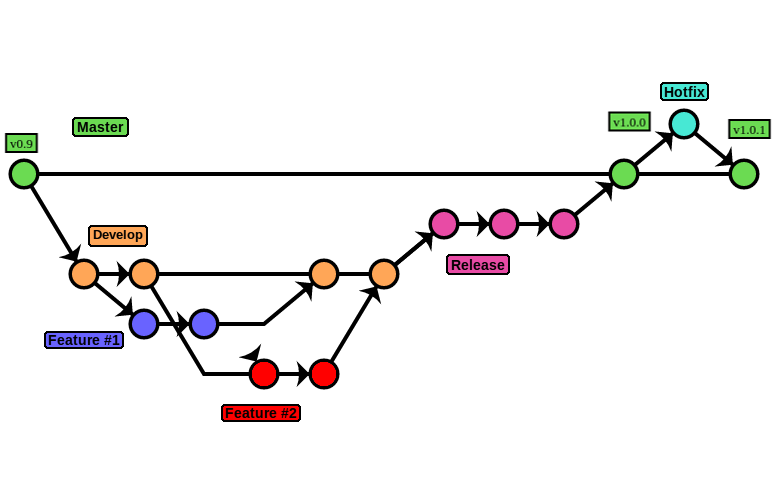
\includegraphics[width=\textwidth]{Resources/Gitflow.png}
\caption{\textit{Gitflow} o flujo de trabajo de Git}
\end{figure}

GitHub es una plataforma de desarrollo colaborativo que te permite alojar tus repositorios Git. Su uso es gratuito si el código almacenado es público. Además, te permite tener una wiki y una página web para tu proyecto, junto a otras funciones.
Una de sus funciones estrella es la visualización online del repositorio, con la que cualquier persona tiene acceso al código y los archivos antes de descargarlos. Otra función útil es el apartado de \textit{Issues}, en el que los usuarios de tu código pueden reportar los bugs del programa o aportar nuevas ideas en forma de "foro".
Tanto el programa como este documento están disponibles en GitHub en los siguientes enlaces. \url{https://github.com/daviddavo/InvProy} y \url{https://github.com/daviddavo/InvProy-tex}

\subsection{LaTeX}
\LaTeX\space o, en texto plano, LaTeX, pronunciado con la letra griega 
Ji ($\Chi$), es un software libre orientado a la creación de textos escritos comparable a la calidad tipográfica de las editoriales. Mediante la importación de paquetes y comandos o macros se puede dar formato al texto al igual que con cualquier otro editor, exportándolo posteriormente a PostScript o PDF. Está orientado a documentos técnicos y científicos por su facilidad a la hora de incluir fórmulas o código e importar paquetes que cumplan las necesidades de los usuarios. No es un procesador de textos, pues está más enfocado en el contenido del documento que en la apariencia de éste.
El código del documento puede ser editado con cualquier editor de texto plano como \textit{nano} o \textit{emacs}, aunque he usado una \acrshort{IDE} llamada \textbf{texmaker}.

\subsection{Python}
Es un lenguaje de programación interpretado (sólo se traduce  el programa a código máquina cuando se debe ejecutar esa parte del código, por lo que no hace falta compilarlo) que destaca porque sus programas poseen una sintaxis más legible que la de el resto de lenguajes. Soporta tanto \gls{programacion imperativa} como programación orientada a objetos. Usa variables dinámicas, es multiplataforma, y, además, es de código abierto, lo que permite distribuir el programa en Windows al distribuir los binarios de Python junto a él. En este proyecto, la versión de Python utilizada es la 3.4 en adelante.

\subsection{Gtk+}
Es un conjunto de bibliotecas o \glspl{Libr} (conjunto de funciones y clases ya definidas preparadas para el uso de los programadores) desarrollado por la GNOME foundation destinado a la creación de Interfaces Gráficas de Usuario (\acrshort{GUI}), también, al igual que Linux forma parte del proyecto GNU.

Contiene las bibliotecas de GTK, GDK, ATK, Glib, Pango y Cairo; de las que he usado fundamentalmente GTK para crear la interfaz principal del programa; \textbf{GDK} al utilizarlo como intermediario entre los gráficos de bajo nivel y alto nivel y \textbf{Cairo} para la creación de algunos de los elementos gráficos del programa.

Al utilizar este conjunto de librerías, se ha conseguido que sólo sea necesario descargar una dependencia del programa, que además suele venir instalada en la mayoria de distros de Linux. Por ejemplo en una instalación limpia de Ubuntu 16 (sin descargar paquetes adicionales) el programa funciona perfectamente. Para usarlo en Python se ha tenido que importar la libreria de PyGtk, que también suele venir incluida en la distribución.

\subsection{Wireshark}
\label{wireshark}
Wireshark es un \textit{packet sniffer} o analizador de paquetes; te muestra los paquetes de red reales enviados y recibidos por una tarjeta de red, lo que facilita la creación del simulador de redes. También te separa las distintas partes de la encapsulación del paquete y además te permite buscar entre los paquetes de red añadidos y recibidos, pudiendo añadir filtros de búsqueda para los distintos campos del paquete y para las distintas capas.

\newpage
\section{Fundamentos básicos de programación}
Una variable no es más que un hueco en la memoria del ordenador, reservado para algo que queremos recordar. Así, podemos establecer una variable llamada `pi' con valor $\mathsf{3.1415...}$, para que luego, en una función, en lugar de escribir `3.14...' múltiples veces, sólo haga falta escribir `pi'. Esto es un ejemplo bastante básico, ya que las variables pueden ser también valores booleanos\footnote{Valores del álgebra de Boole; Verdadero/Falso, 1/0, True/False...}, listas, diccionarios (listas de tipo clave:valor), objetos, series de carácteres...
Las variables se establecen así: \mintinline{python3}|variable = valor|.

Una función, es un conjunto de instrucciones, que, dados unos argumentos (o ninguno) realiza una serie de acciones y/o retorna información (un número, objeto, valor, etc.). Por ejemplo, podríamos crear una función \texttt{sum(a,b)}, que dados dos números, retorne la suma de estos. Se dice `llamar a una función' cuando se le da al programa la instrucción de que ejecute la función. Para ello, usamos \mintinline{python3}|funcion(argumento1,argumento2...)|. Los argumentos pueden ser cualquier cosa, desde una variable binaria (1 o 0, Verdadero o Falso) a un Objeto. Además, al terminar una función retorna un valor; que puede ser usado si la función es llamada para establecer una variable. (P.ej: \mintinline{python3}|sumatorio = sum(3, 8)|

Las clases sirven para crear objetos, por ejemplo, un Switch, un cable, una ventana, o una dirección MAC son objetos. Las clases, contienen variables y funciones. Las variables pueden ser distintas para cada objeto, mientras que las funciones son las mismas. Así todos los conmutadores tienen una función que actúa cuando reciben un paquete, pero cada uno posee una dirección MAC distinta, unas coordenadas distintas, un nombre distinto... Para crear un objeto, simplemente tenemos que `llamar' a la clase mediante una variable, p.ej: \mintinline{python3}|objeto = Clase()|. Como la función que crea el objeto también acepta argumentos, hay objetos que necesitan argumentos para ser creados (\mintinline{python3}|P = punto(5,7)|. También, podemos establecer variables de objeto: \mintinline{python3}|objeto.nombre = "Objeto Guay"|.

Al final, todo programa se basa en condiciones y funciones. ``Si ocurre esto, haz esto otro; si no ocurre, haz aquello". Para ello, se simplifica cualquier expresión en VERDADERO o FALSO, parecido a la lógica aristotélica. Si la expresión dada es verdadera, se ejecutará el código de dentro del condicional. También existe la expresión \texttt{elif}, donde se especifica otra condición, que se ejecutará en caso de que no se cumpla la anterior pero sí esta; y la expresión \texttt{else}, en caso de que no se cumpla ninguna de las anteriores.
\begin{minted}[baselinestretch=1,	linenos,
	breaklines
	]{python3}
if condicion:
  funcion()
elif condicion2:
  funcion2()
elif condicionN:
  funcionN()
else:
  print("Algo no funciona")
\end{minted}
En condición, puede haber cualquier expresión que pueda ser verdadera. Las que unen condiciones son \texttt{and} y \texttt{or}, en lenguaje matemático, intersección y unión. Y las condiciones suelen ser expresiones matemáticas, como a > b, a >= b, a == b, o a != b. Aunque en ocasiones pueden usarse con otros tipos de variables, como las series de caracteres. Por ejemplo \mintinline{python3}|if entrada == "Yes":|, en la que si la variable \texttt{entrada}, que hemos definido anteriormente como texto introducido por el usuario, es igual a "Yes", ejecutaremos código. En mi programa tiene aplicaciones como `Si el objeto es un conmutador' o `si la coordenada x buscada es igual a la coordenada x del objeto y la coordenada y buscada es igual a la coordenada y del objeto'.

Ahora, veremos un pequeño ejemplo práctico, que junta todo:
\begin{minted}[baselinestretch=1,linenos,
	breaklines
	]{python3}
def esnatural(numero): #Definimos la función, asumiendo que no hay números complejos
  absoluto = abs(numero) #Absoluto es igual al resultado de la función absoluto del numero
  entero   = int(numero) 
  if absoluto == entero: #Si el número absoluto es igual al entero.
    print("Es un número Natural") #Ponemos eso en la consola
    return True
  elif numero == entero: #No es positivo, por lo que miramos a ver si es negativo, pero entero.
    print("Es un numero Entero, pero no Natural")
    return False
  else:
    print("Es un numero Racional")
    return False
\end{minted}

\section{Fases del desarrollo de software}
Durante el desarrollo de software existen distintas fases, desde el comienzo hasta el lanzamiento del programa.
\subsection{Estadios de desarrollo}
\begin{description}
\item \textbf{Pre-alpha:} Todas las actividades realizadas antes de las pruebas formales. Actividades como diseño, programación, análisis de requisitos... En software libre, hay distintos tipos de versiones pre-alpha. Se añaden funcionalidades al software.
\item \textbf{Alpha:} Se añaden más funcionalidades al software. El software es inestable (tiene muchos \textit{bugs}) y puede causar pérdidas de datos. Normalmente aún no está disponible para el uso por usuarios; aunque, en software libre, la versión Alpha suele estar ya disponible para el público. Esta fase termina cuando se hace una `\textbf{congelación de funcionalidades}, es decir, se determina que ya no se van a añadir más funcionalidades a la versión.
\item \textbf{Beta:} Se inicia esta fase cuando el programa se considera \textbf{completo de funcionalidades} (cuando se hace una congelación). Aún así el programa puede contener muchos \textit{bugs} conocidos o desconocidos, además de problemas de rendimiento y cuelgues. Se prueba el programa con tests de usabilidad.
Aquí ya se publica una versión para el usuario, denominada \textit{Beta Release}, en ocasiones también es llamada \textbf{TP}(\textit{Technical preview} o avance técnico). En ocasiones, como en algunos programas de software libre, el programa se mantiene en fase Beta y nunca se dejan de añadir funcionalidades. Se considera beta abierta si la versión está disponible al público, y beta cerrada en caso contrario.
\item \textbf{RC}: \textit{Release Candidate}. Es una versión beta que tiene el potencial de convertirse en una versión final del programa, que está lista para lanzar si no surgen \textit{bugs} importantes. En esta fase se estabiliza el programa y se prepara para el lanzamiento con numerosos tests.
\end{description}
\subsection{Publicación}
Cuando el programa es publicado, la versión del programa se considera `versión estable'.
\begin{description}
\item \textbf{RTM:} \textit{Release to manufacturing} o Versión para producción, también llamada `gold master' o `versión de oro'.  Es la versión que va a ser enviada al centro de distribución, se eliminan archivos de funcionalidades de pruebas y se hacen muchas comprobaciones de la integridad de los archivos.
\item \textbf{GA:} \textit{General availability} o disponibilidad general. Fase en la que se produce el \textit{marketing} y la venta del programa. Éste ya está disponible para su compra, dependiendo de la región, el idioma, o el método de adquisición del programa (DVD, BD, Web).
\end{description}
\subsection{Soporte}
Después de ser lanzada una versión de un programa, durante un tiempo denominado `tiempo de vida' la versión aún tiene soporte oficial, en el que se pueden aplicar todavía actualizaciones de servicio y parches para solucionar \textit{bugs} o, en ocasiones, incluir nuevas funcionalidades.
\begin{description}
\item \textbf{Fin de soporte:} Cuando la versión deja de ser distribuida y se deja de dar soporte, se dice que ha alcanzado el `fin de vida', o pasa a ser obsoleto, retirado o descontinuado. A pesar de esto, la gente puede seguir queriendo usar el programa, como con Windows XP.
\end{description}

\definecolor{chaptercolour}{HTML}{051C38}
\definecolor{sectioncolour}{HTML}{143153}
\definecolor{subsectioncolour}{HTML}{4B688B}
%\definecolor{subsubsectioncolour}{HTML}{CDB380} %TERRA
\definecolor{subsubsectioncolour}{HTML}{748BA7}
\chapter{Redes Informáticas}
\section*{Historia}
El uso de redes informáticas nace en la década de 1960, para suplir la necesidad de las universidades y laboratorios de investigación de conectar los distintos ordenadores. En la década de 1970 se comienza a experimentar con tecnologías de redes LAN, algunas de ellas usadas actualmente o recientemente, como Ethernet, desarrollado en 1975 por Xerox PARC (Palo Alto Research \& Development). 

Las redes se usaban sobre todo para aprovechar el almacenamiento y las impresoras. Cada vendedor incluía su propio tipo de tarjeta de red, cableado, protocolo y sistema operativo de red, hasta que Novell NetWare (Sistema Operativo de red desarrollado por Novell inc.) salió al mercado en 1983 soportando la mayoría de tipos de tarjetas de red y cables. Fue el SO de Red dominante hasta que en 1993 Microsoft lanzó Windows NT AS y Microsoft Windows para Trabajo en Grupo. Al mismo tiempo, los dispositivos Unix usaban sistemas basados en TCP/IP.

Actualmente el protocolo TCP/IP es considerado un estándar y ha reemplazado el resto de protocolos usados hasta principios de los 2000.

\newpage

\section{Capas de Red/Modelo OSI}
El modelo \acrshort{osi} es un modelo de referencia para redes basado en \gls{capas de abstraccion}.
Su objetivo es conseguir la interoperabilidad entre sistemas haciendo uso de los protocolos estandarizados. Fue creado en 1980 por la Organización Internacional de Estandarización (\acrshort{iso}). No es considerado una arquitectura de red porque los protocolos no forman parte del modelo, sino que son entidades de distintas normativas internacionales.
\definecolor{odd}{HTML}{FFFFFF}
\definecolor{even}{HTML}{E0E0E0}
\definecolor{header}{HTML}{42A5F5}
\vspace*{5pt}

\rowcolors{1}{header}{header}
\rowcolors{2}{odd}{even}
\renewcommand{\arraystretch}{1} %Antes 1.1
\noindent\linespread{1}
\begin{tabularx}{\linewidth}{ | l >{\footnotesize}c >{\footnotesize}X >{\footnotesize}c | }
	\rowcolor{header} \hline
	\textbf{Capa} & \textbf{PDU\footnote{\textit{Protocol Data Unit} o Unidad de Datos de Protocolo.}} & \textbf{Función} & \textbf{Ejemplos} \\ \hline
	1. Física & Bit & Transmisión y recepción de bits físicos sobre un medio físico (topología de red) & 	 RJ45, IEEE 802.11, etc. \\
	\label{osi}
	2. Data Link & Frame & Transmisión segura de \textit{frames} entre dos nodos conectados por una capa física. & Ethernet, 802.11, etc...\\
	3. Red & Paquete & Estructurar y administrar una red multinodo. Incluye enrutamiento, control de tráfico, y asignación de direcciones & IPv4, IPv6, ICMP... \\
	4. Transporte & \begin{tabular}[t]{@{}c@{}}Datagrama(UDP)\\Segmento(TCP)  \end{tabular} &
	Transmisión de segmentos de datos entre los puntos de una red, incluyendo ACK & TCP, UDP...\\
	5. Sesión & Datos & Administración de sesiones de comunicación, como intercambio continúo de información entre dos nodos. & SSH, RPC, PAP...\\ 
	6. Presentación & Datos & Translación de datos entre un servicio de red y una aplicación. Incluye comprensión, encriptación/decriptación, y codificación de carácteres. & MIME, TLS \\
	7. Aplicación & Datos & APIs de alto nivel, incluyendo recursos compartidos y acceso remoto de archivos & HTTP, FTP, SMTP... \\ \hline
\end{tabularx}

\newpage
\section{Topologías de red}
\label{topdred}
La \gls{topologia} de red es la configuración de los elementos que componen una red. Puede ser representada lógica o físicamente. \\
La topología lógica puede ser igual en dos redes, aunque su topología física (distancia entre conexiones, tipo de señales...) pueda ser distinta. Se distinguen dos elementos: los nodos (distintos dispositivos de red) y los enlaces (medio de transmisión de los datos).
\subsection{Clasificación de las topologías de red}
Se distinguen ocho tipos de topologías de red: \cite{bicsi-02}
\renewcommand{\labelitemi}{$\bullet$}
\begin{description}
\item \textbf{Punto a punto:} conexión directa entre los dos puntos de la red. También es conocida como \textit{P2P} (\textit{Peer to Peer}).
\item \textbf{Estrella:} cada nodo está conectado a un nodo central que puede ser un enrutador, concentrador o conmutador.
\item \textbf{Bus:} cada nodo está conectado a un único cable. Una señal de un dispositivo viaja en ambos sentidos por el cable hasta que encuentra el destino deseado.
\item \textbf{Anillo:} es una topología en bus pero con los extremos conectados. Los datos atraviesan el anillo en una única dirección y van atravesando cada uno de los nodos, por lo que si uno de ellos no funciona, la red tampoco.
\item \textbf{Malla:} se pueden distinguir dos tipos: completamente conectados, en la que todos los nodos están conectados entre ellos, y parcialmente conectados, en la que algunos nodos pueden estar conectados punto a punto y otros pueden tener varias conexiones.
\item \textbf{Híbrida:} combinan dos o más topologías. La más famosa es la topología de \textbf{árbol}, en la que se conectan varias topologías de estrella, asemejando la forma de un árbol.
\item \textbf{Cadena:} se conecta cada ordenador en serie con el siguiente. Cada ordenador repite el mensaje al siguiente ordenador si éste no es su destino. Si se cierra el circuito se crea una topología en anillo, mientras que si se deja abierto se denomina topología lineal.
\end{description}

\begin{figure}[H]
\centering
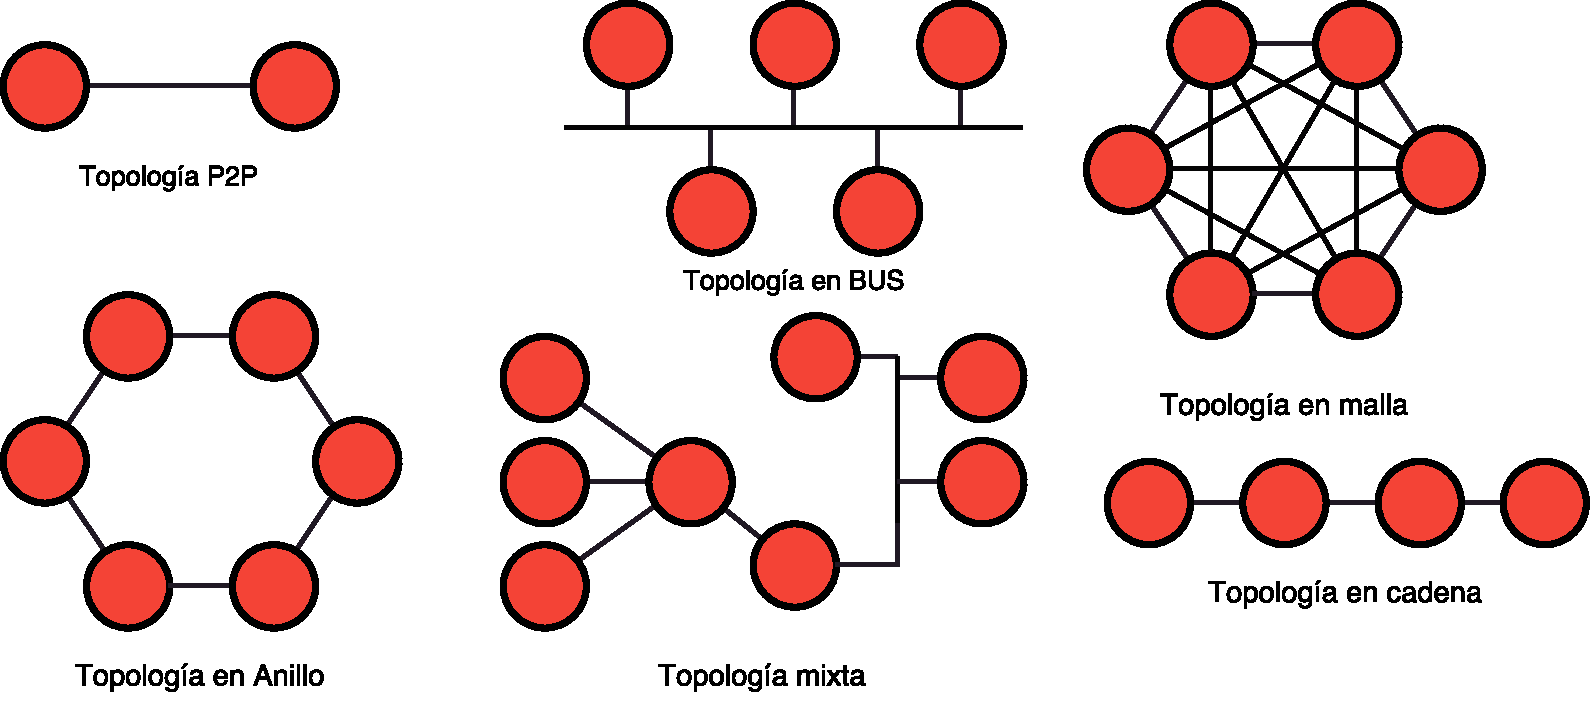
\includegraphics[width=\textwidth]{Resources/Top/Topdered.pdf}
\caption{Representación esquemática de las diferentes topologías de red.}
\end{figure}

\subsection{Nodos de una red}
\begin{description}
\item \textbf{\textit{Router} o enrutador:} es un dispositivo de red que reenvía los paquetes analizando la capa 3 del modelo OSI (IP) y conecta dos redes.
\item \textbf{Puente de red o \textit{bridge}:} Funciona en la capa 2 del modelo OSI. Es un dispositivo que conecta dos segmentos de red formando una única subred, por lo que las dos ``redes" pueden conectarse e intercambiar datos sin necesidad de un \textit{router}.
\item \textbf{Conmutadores o \textit{switches}:} dispositivo de red que filtra los datagramas del nivel 2 OSI (\textit{Data Link Layer}, ver \ref{osi}, pág. \pageref{osi}), también conocidos como \textit{frames}, y reenvía los paquetes recibidos entre los puertos, dependiendo de la dirección MAC de cada datagrama. La diferencia entre un conmutador y un concentrador es que el conmutador sólo reenvía los paquetes por el puerto necesario. También existen un tipo especial de conmutadores que pueden hacer uso de la capa 3 OSI.
\item \textbf{Repetidores y concentradores:} un repetidor es un dispositivo de red que, llegada una señal, limpia el ruido innecesario y la regenera. Un repetidor con múltiples puertos es un concentrador o \textit{hub}, trabajan en la capa 1 del modelo \acrshort{osi}. Los repetidores requieren de un pequeño tiempo para regenerar la señal, lo que puede crear un retardo en el tiempo de envío de la señal.
\item \textbf{Interfaces de Red:} también conocido como tarjeta de red o \textit{Network Interface Controller} (NIC), es un \gls{hardware}, normalmente integrado en la placa base, que permite al ordenador conectarse a una red. Recibe el tráfico de una dirección de red. En las redes que hacen uso de Ethernet, tiene una dirección de Control de Acceso al Medio (\acrshort{MAC}) única. Estas direcciones son administradas por el Instituto de Ingeniería Eléctrica y Electrónica (\acrshort{IEEE}) evitando la duplicidad de estas. Cada dirección MAC ocupa 6 octetos, o 48 bits, a lo que suele ser representada como una cadena hexadecimal, por ejemplo: ``4C:33:31:64:59".
\item \textbf{Módem:} Dispositivos que transforman señales analógicas a digitales y viceversa. Son usados mayoritariamente en el \acrshort{ADSL}.
\item \textbf{Cortafuegos o \textit{firewalls}:} dispositivo que controla la seguridad mediante reglas de acceso. Aceptan determinados paquetes mientras rechazan otros. En una red doméstica, se puede poner un firewall que sólo acepte tráfico de los puertos de uso común (Páginas Web, e-mail, etc.) y rechace otros más peligrosos (Acceso remoto, SSH, SMTP, SOCKS...).
\end{description}

%\subsection{Enlaces de red}
Según el modelo OSI, los enlaces de red corresponden a las capas 1 y 2. El medio físico puede ser tanto ondas de radio (Wi-Fi), como fibra óptica (FTTH) o impulsos de red (PLC, Ethernet, DSL).

\subsubsection{Cableado}
\begin{description}
\item \textbf{Coaxial:} Cables de cobre o aluminio recubiertos de aislante, rodeado de un conductor, así se reducen las interferencias y la distorsión. Normalmente son usados para la transmisión de radio y TV, pero pueden ser usados para redes informáticas. Pueden llegar hasta a 500 Mbit/s.
\item \textbf{Par trenzado o \textit{Ethernet}:} Es el más usado en redes locales. Es un cable formado por finos cables trenzados en pares. En telefonía se usa el RJ11 o 6P4C (6 posiciones, 4 conectores) formado por 2 pares. Para ordenadores, según el estándar \textit{Ethernet} se usa 8P8C o RJ45 de 4 pares, debido al nombre del estándar, este cable suele ser comúnmente llamado "cable de Ethernet". Puede llegar hasta 10 Gbit/s
\item \textbf{Fibra óptica:} Hilo de cristal o plástico flexible que permite que la luz se refleje en su interior, transmitiéndola de un extremo a otro del cable. No tienen apenas pérdida por distancia y son inmunes a las interferencias electromagnéticas. Además, permiten varias frecuencias de onda, lo que equivale a una transferencia de datos más rápida. Son usados para salvar las largas distancias entre continentes.
\end{description}

\subsubsection{Comunicación inalámbrica o \textit{Wireless}}
\begin{description}
\item \textbf{Microondas terrestres:} Transmisores, receptores y repetidores terrestres que operan en frecuencias de entre 300 MHz y 300 GHz de propagación de alcance visual, por lo que los repetidores no se separan más de 48 km.
\item \textbf{Comunicación satelital:} Microondas y ondas de radio que no sean reflejadas por la atmósfera terrestre. Los satélites mantienen una órbita geosíncrona, es decir, el periodo de rotación es el mismo que el de la tierra, lo que se produce a una altura de $\mathsf{~35786}$ km.
\item \textbf{Celular o PCS:} Ondas electromagnéticas de entre 1800 y 1900 MHz. Son las usadas por los teléfonos móviles. A partir del 2G o GPRS, se podia acceder a Internet con de TCP/IP. El sistema divide la cobertura en áreas geográficas, cada una con un repetidor. Repiten los datos entre un repetidor y el otro.
\item \textbf{Ondas de radio:} Ondas de 0.9, 2.4, 3.6, o 5 GHz. El estándar más usado es el \textit{IEEE 802.11}, también conocido como wifi o Wi-Fi que opera en la banda de 2.4 GHz, a excepción de la versión IEEE 802.11ac que opera a 5GHz que tiene menos interferencias, pero también menor alcance.
\end{description}
\newpage
\section{Paquetes de red}
Son cada serie de bits en los que se divide la información enviada por una red. \\ Según el modelo OSI, un paquete es estrictamente el PDU de la capa de red. El paquete de red se encuentra encapsulado en la capa anterior del modelo OSI. Por ejemplo, en éstandares de comunicación TCP/IP, un segmento TCP puede ser llevado por varios paquetes IP transportados por varios frames de Ethernet. \\Está formado por varios protocolos y en él se distinguen tres partes:
\begin{description}
\item \textbf{Header} o cabecera: Datos e información sobre el paquete. (Dirección IP, MAC, etc)
\item \textbf{Payload} o carga: Los datos que se quieren transferir.
\item \textbf{Trailer} o cola: En ocasiones es inexistente (como en UDP) pero suele ser un código de comprobación de errores.
\end{description}
\vspace*{0.5cm}
\begin{figure}[H]
\noindent
\centering
\includegraphics[width=\textwidth]{Resources/Encapsulación_OSI.pdf}
\caption{Encapsulación de red. El Datagrama IP es lo considerado 'Paquete de red'}
\end{figure}
\newpage

\section{Protocolos}
Un protocolo de comunicación es un conjunto de reglas para intercambiar información entre enlaces de red. En una pila de protocolos, cada protocolo cubre los servicios del protocolo de la capa anterior. Por ejemplo, un e-mail se envía mediante el protocolo \acr{POP3} en la capa de Aplicación, sobre TCP en la capa de transporte, sobre IP en la capa de Red, sobre Ethernet para la capa \textit{Data Link}. Para entenderlo mejor, es como la gramática de la lengua. Un sustantivo forma parte de un sintagma nominal, que forma parte de un sujeto, que a su vez forma parte de una oración. Siendo las ondas sonoras producidas la capa física.
\begin{figure}[H]
\noindent
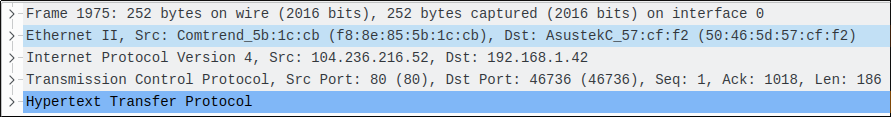
\includegraphics[width=\textwidth]{Resources/Wireshark01.png}
\caption[Captura de pantalla de Wireshark]{Captura de pantalla de Wireshark (Véase \ref{wireshark}, pg. \pageref{wireshark}) en la que se muestran los protocolos que forman un paquete de red HTTP.}
\end{figure}

\subsection{Familia de protocolos de internet}
También conocido como \textit{Internet Protocol Suite}, y más conocido como TCP/IP, es el fundamento de las redes informáticas. Se trata de un conjunto de más de 100 protocolos que permiten la conexión de ordenadores tanto en Internet como en LAN, incluyendo protocolos de las aplicaciones más usadas.

\setcounter{secnumdepth}{5}
\subsubsection{Aplicación}
Es la capa en la que se envían los datos a otras aplicaciones en otro ordenador o en el mismo. Las aplicaciones hacen uso de las capas inferiores para asegurarse que los datos lleguen a su destino. Algunos de los protocolos más usados son:
\begin{itemize}
\item \textbf{HTTP} \textit{Hypertex Transfer Protocol:} Protocolo de Transferencia de Hipertexto. Es el protocolo base de la World Wide Web. Se trata de texto estructurado que usa hiperenlaces entre nodos que también contienen texto. El cliente, al entrar en una \acr{url}, el agente de usuario (navegador) envía al servidor una petición de la página web, mediante HTTP. El servidor, envía como respuesta un documento HTML u otro recurso.
\item \textbf{DNS} \textit{Domain Name System:} Sistema de Nombres de Dominio. Un servidor DNS almacena una base de datos distribuida y jerárquica con información sobre el nombre del dominio y la dirección IP a la que está vinculada. Al intentar conectar a  \texttt{http://www.4chan.org}, el cliente pregunta al servidor cual es la dirección IP asociada a esa dirección, y se conecta a tal IP, en este caso 104.16.66.203. Para evitar tener que consultar continuamente con el servidor, se almacenan en una \gls{cache} en el cliente.
\item \textbf{TLS/SSL} \textit{Transport Layer Security}, y su predecesor \textit{Secure Sockets Layer} (Ver \ref{seguridad}).
\item \textbf{HTTPS} HTTP Seguro. Es HTTP con TLS aplicado.
\item \textbf{DHCP} \textit{Dynamic Host Configuration Protocol}: Protocolo de configuración dinámica del host. Este protocolo es controlado por un servidor DHCP que envía parámetros de configuración automática a los clientes. El ejemplo más común es el de cualquier Router doméstico, que asigna automáticamente a cada dispositivo una dirección IP diferente, pero dejando un rango en el que se pueden establecer IP's estáticas.
\item \textbf{FTP} \textit{File Transfer Protocol:} Protocolo de Transferencia de Archivos, te permite enviar archivos entre un cliente y un servidor. El protocolo TLS aplicado a FTP se denomina FTPS. Te permite acceder, mediante un usuario y contraseña, o de forma anónima, a un sistema de archivos jerárquico con nombres de archivo codificados. Utiliza el puerto 21 de forma predeterminada.
\item \textbf{SSH} \textit{Secure Shell:} Terminal seguro. Es un protocolo de red criptográfico que permite a un cliente conectarse a un servidor y ejecutar comandos de terminal como un usuario (conociendo el usuario y contraseña). Además, permite la creación de túneles, lo que permite asegurar cualquier aplicación a través de SSH, y el acceso a puertos bloqueados por el cortafuegos en el cliente. La mayoría de servidores de SSH incluyen un servidor de SFTP, el protocolo FTP con SSH aplicado.
\item \textbf{IMAP} \textit{Internet Message Access Protocol:} Protocolo de acceso a mensajes de Internet. Usa una conexión TCP/IP para conectarse a un servidor de e-mail y ver el contenido de los mensajes, sin necesidad de descargarlos. A diferencia de POP, te permite usar una bandeja de entrada desde varios clientes.
\end{itemize}
\subsubsection{Transporte}
Se encapsulan los datos de aplicación en un segmento o datagrama, dependiendo si el protocolo usado es TCP o UDP. Se encarga de transportar los datos por una red independientemente de la red física.
\begin{itemize}
\item \textbf{TCP} \textit{Transmission Control Protocol:} Protocolo de Control de Transmisión. Se aplica a los paquetes para administrarles un orden y un sistema de comprobación de errores. Con todas las funcionalidades, ocupa bastante espacio, lo que aumenta la latencia, aunque es más fiable para el envío de la mayoría de los datos.
\item \textbf{UDP} \textit{User Datagram Protocol:} Es un protocolo muy minimalista. A diferencia del TCP, no garantiza que los paquetes lleguen, o lleguen en orden, o protección ante duplicados. Reduce mucho la latencia ya que no usa \textit{handshaking}. Por ello es usado por ejemplo para \textit{streamings} de televisión o videollamadas.
\end{itemize}
\subsubsection{Red}
El objetivo es que los datos lleguen del origen al destino, aún cuando no están conectados directamente. Los enrutadores o \textit{routers} son los dispositivos que cumplen esta función.
\begin{itemize}
\item \textbf{IP} \textit{Internet Protocol}: Protocolo de Internet. Envía datagramas o paquetes de red a través de redes. Tiene una función de enrutamiento que es la que permite la interconexión de redes, y la existencia de Internet. Es un protocolo que encapsula el paquete definiendo en el \textit{header} (cabecera) las direcciones IP del servidor y el cliente, o remitente y destinatario. La versión usada actualmente es IPv4 desarrollado en 1981, pero poco a poco se va abriendo paso la versión IPv6. La mayor diferencia es que la versión cuatro cuenta con direcciones de 32 bits lo que permite tan sólo unas 4.3 millardos ($\mathsf{2^{32}}$) de direcciones, mientras que la versión 6 tiene direcciones de 128 bits, lo que permite más de 340 sextillones ($\mathsf{2^{128}}$)de direcciones
\item \textbf{ICMP} \textit{Internect Control Message Protocol}: Es un protocolo que no es usado por aplicaciones de usuario (a excepción de herramientas de diagnóstico como ping o traceroute). Lo usan los dispositivos de red, como los routers, para enviar notificaciones o mensajes de error indicando que un servicio no está disponible.
\end{itemize}
\subsubsection{Link}
Capa encargada del acceso al medio físico de la red. También cumple otras funciones como incluir una comprobación de errores e identificar cada dispositivo de forma única.
\begin{itemize}
\item \textbf{ARP} \textit{Address Resolution Protocol:} Protocolo de resolución de direcciones. Es un protocolo que convierte direcciones de la capa de Red a la capa de Enlace (dir. IP a dir. MAC). El dispositivo, al conectarse una red, envía un \textit{frame} ARP con su dirección MAC y su IP, para que los demás dispositivos de la red lo almacenen en su memoria y poder usar ambas direcciones al enviar un paquete.
\item \textbf{MAC} \textit{Media access control}: Control de acceso al medio. Es un conjunto de protocolos (Como Ethernet o IEEE 802.11 [WiFi]) encargados de asignar el medio físico de la red. Evita colisiones entre paquetes asegurándose de que el medio está libre y evitando así la transmisión simultánea.
\end{itemize}

\section{Seguridad de redes}
\label{seguridad}
Consiste en el conjunto de acciones que toma el administrador de redes para prevenir y evitar acceso no autorizado, mal uso, o caída del servicio de red.
\subsection{Tipos de ataques}
Hay dos tipos de ataques de red, los activos y los pasivos. Son ataques pasivos cuando el intruso intercepta los datos que viajan por la red, y se considera activo cuando el atacante modifica el funcionamiento normal de la red.

Algunos de los ejemplos de los ataques más comunes son:

\begin{easylist}[itemize]
\ListProperties(Style*=$\bullet$ , Style2*=--)
& \textbf{Ataques pasivos}
&& \textbf{Sniffing o analizador de paquetes:} Mediante un software se muestran los datos de los paquetes de red enviados y recibidos por la red.
&& \textbf{Escáner de puertos:} Se envían numerosas peticiones al servidor por los servidores más comunes, así se comprueba que puertos están abiertos. Por ello es recomendable cambiar los puertos por defecto de los servidores importantes.
&& \textbf{Escáner IDLE:} Se realiza un escáner de puertos para saber que servicios están disponibles, pero a traves de otro ordenador "zombie", y observando el comportamiento de éste.
& \textbf{Ataques activos}
&& \textbf{Ataque de Denegación de Servicio:} Se ``desborda`` el ancho de banda mediante el envío de muchas peticiones a un servidor, además de ser de un tamaño excesivo.
&& \textbf{Ataque DDoS:} \textit{Distributed Denial of Service}, o un ataque de Denegación de Servicio distribuido. Varios ordenadores hacen un ataque DoS a un mismo servidor, algunas veces los ordenadores forman parte de una \gls{botnet}, y en ocasiones ocurre sin querer (al haber demasiado tráfico de red).
&& \textbf{Phishing:} Con el objetivo de obtener información como nombres de usuario y contraseña o tarjetas de crédito, se crea una página de apariencia parecida a la página que trata de simular. Los usuarios más incautos no notarán el cambio e introducirán sus datos en esta página.
&& \textbf{SQL Injection:} Es una técnica de inserción de código. Al pedir un servidor SQL datos como ``Nombre`` o ``Apellido``, se introduce junto a estos código malicioso que el servidor puede ejecutar. Por ejemplo, \mintinline[breaklines]{SQL}|SELECT * FROM alumnos WHERE nombre = '<nombreintroducido>' ;|. <nombreintroducido> puede ser \texttt{Pablo} o \texttt{Juan}, pero si se introduce \texttt{x'}\mintinline[breaklines]{SQL}|; DROP TABLE alumnos; SELECT * FROM asignaturas WHERE 't' = 't'|, el código que interpreta el servidor eliminaría la tabla \texttt{alumnos} por completo.
&& \textbf{Ataque Smurf:} Es una especie de ataque DDoS. Se envían paquetes ICMP (probablemente pings) a distintas máquinas, pero estos paquetes que se envían, el valor de la dirección IP del remitente es la dirección IP del objetivo al que se quiere atacar. Por lo que, las máquinas a las que se las ha enviado el mensaje ICMP responderán todas al objetivo, haciendo así un DDoS.
&& \textbf{DNS poisoning:} Se modifica la caché de DNS de un ordenador, redireccionando a una IP incorrecta, de esta manera se puede realizar un ataque de phishing sin que lo sepa el usuario del ordenador. En el caso de hacerlo con las tablas de ARP, se denomina \textit{ARP Poisoning}.
\end{easylist}
\subsection{Contramedidas}
Acciones que se pueden tomar para evitar algunos de los ataques de red más comunes.
\subsubsection{Encriptación}
Se suele denominar también E2EE o \textit{End-to-end encryption}, es decir, encriptación de punto a punto.\\
Se suelen usar claves PGP (\textit{Pretty Good Privacy}, Privacidad bastante buena) para cifrar correos electrónicos y otros archivos. Para HTTP lo más común es la encriptación TLS, aunque también se está utilizando actualmente para email. El servidor genera o contiene una clave o certificado, luego el cliente, debe recibir o tener esa clave para poder desencriptar el mensaje.
\subsubsection{Cortafuegos}
Primero necesitamos definir lo que es un \textbf{puerto}. Un puerto es un punto final de comunicación en un Sistema Operativo. El puerto siempre está asociado a una dirección IP y a un tipo de protocolo. Así completa el origen o destino de un paquete de red. Se aplica en la capa de transporte del modelo OSI. El puerto es un número de 16 bits, por lo que será un número comprendido entre 0 y 65536. Multitud de puertos están ya reservados por diversos protocolos y programas, como el 80 para HTTP, 22 para SSH o 25 para SMTP.

Un cortafuegos es un software que supervisa el tráfico de entrada y salida de datos, basado en unas reglas. Si un paquete de red cumple esas reglas, es rechazado. Pueden bloquear un paquete destinado a un puerto, de un protocolo (Bloquear SSH de Internet, pero no local), de una IP específica, entre otros atributos. También pueden configurarse en modo negativo o whitelist, aceptando tan sólo los paquetes que cumplan las reglas. Por ejemplo, puedes especificar que no acepte tráfico en el puerto 23. Pero igualmente puedes especificar que sólo acepte tráfico en el puerto 23.

%\begin{figure}[H]
%\noindent
%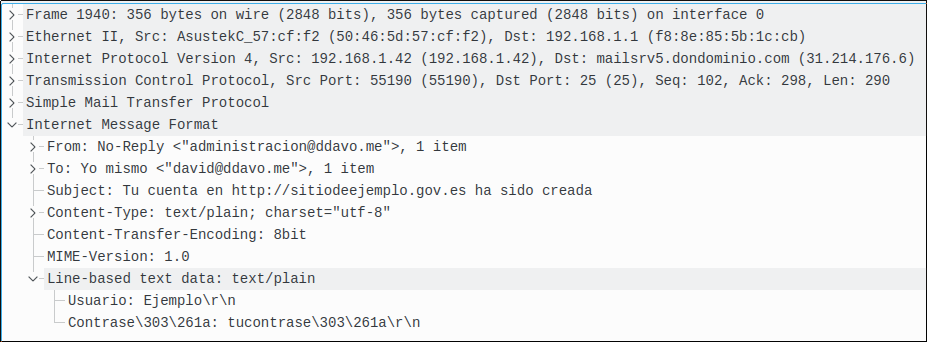
\includegraphics[width=\textwidth]{Resources/Wireshark02.png}
%\caption[Wireshark: SMTP sin encriptación]{Captura de pantalla de Wireshark (Véase \ref{wireshark}, pg. \pageref{wireshark}) en la que se muestra un paquete SMTP (email enviado) sin ningún tipo de encriptación. Se puede acceder a este paquete desde cualquier nodo de la red.}
%\end{figure}
\begin{figure}[H]
\noindent
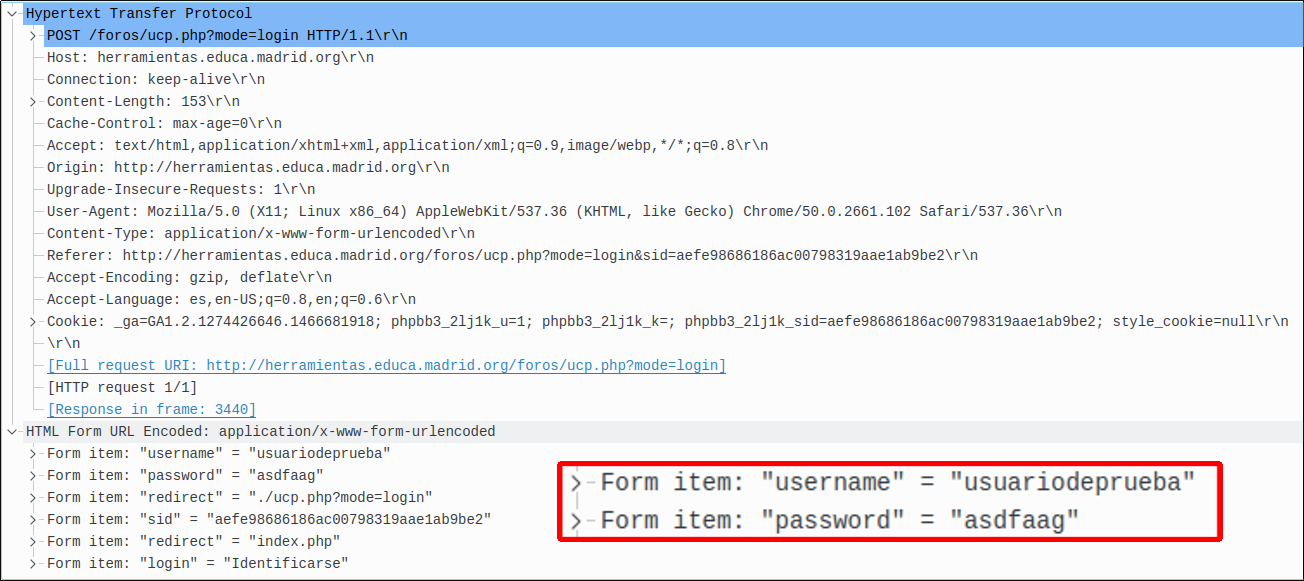
\includegraphics[width=\textwidth]{Resources/Wireshark03.png}
\caption[Wireshark: HTTP Form sin encriptación]{Captura de pantalla de Wireshark (Véase \ref{wireshark}, pg. \pageref{wireshark}) en la que se muestra un formulario de HTTP en el que personas autorizadas podrían ver el usuario y la contraseña.}
\end{figure}

\definecolor{chaptercolour}{HTML}{375000}
\definecolor{sectioncolour}{HTML}{597814}
\definecolor{subsectioncolour}{HTML}{A8C764}
%\definecolor{subsubsectioncolour}{HTML}{CDB380} %TERRA
\definecolor{subsubsectioncolour}{HTML}{D6EF9F}

\newcommand{\function}[1]{\texttt{\color{Orange}#1}}
\newcommand{\class}[1]{\texttt{\color{DarkRed}#1}}
\chapter{El simulador de redes}
La parte práctica del Proyecto de Investigación, el simulador de redes de nombre \textit{InvProy}, ha sido la parte más extensa del proyecto, que más tiempo, esfuerzo y recursos ha ocupado. Se podría decir que el proyecto entero es la parte práctica. Como curiosidad, el nombre de \textit{InvProy} viene del acrónimo formado mediante la permutación de las palabras ``Proyecto de Investigación", quedando \textit{``Investigación \sout{de} Proyecto"} y de ahí \textit{InvProy}.

\section{Instalación}
\subsection{Ubuntu / Debian}
Tan sólo se debe descargar el paquete del programa. Para ello debemos usar apt-get:
\mint{bash}|~ $ sudo apt-get install invproy|

En caso de no estar en los repositorios, hay que hacerlo manualmente. Descarga el paquete de \url{https://github.com/daviddavo/InvProy/releases/latest}. Una vez descargado, abre una terminal donde se haya descargado el paquete e instálelo.
\begin{minted}{bash}
Descargas $ sudo dpkg -i invproy_x.y.z_all.deb
\end{minted}
Donde `x', `y', y `z' son la versión del paquete descargado.
Para iniciar el programa debes usar la lista de programas de tu escritorio.

\subsection{Arch Linux}
Descarga la versión más reciente para Arch Linux de \url{https://github.com/daviddavo/InvProy/releases/latest}. Una vez descargado, abre una terminal donde se haya descargado el paquete e instálelo.
\begin{minted}{bash}
~ $ sudo pacman -S base-devel #Lo necesitas para compilar el paquete
#Ahora elige el sitio donde descargaras el paquete. Aqui no se va a instalar.
~ $ cd Builds
Builds $ curl -O <url> #Lo descargamos
Builds $ tar -xvzf invproy.tar.gz
Builds $ cd invproy
Invproy $ makepkg -sri
\end{minted}

Y ya lo tendrías instalado en tu ordenador.

\subsection{Ejecución manual / instalación portable}
Lo primero que necesitará es descargar las dependencias. Esto depende del Sistema Operativo. En el caso de GNU/Linux, sólo es necesario descargar \texttt{python3-gobject}. Después, clonamos el repositorio de git. Ejemplo en Ubuntu:
\begin{minted}{bash}
~ $ sudo apt-get update && sudo apt-get upgrade
~ $ sudo apt-get install git python3-gobject
~ $ cd Descargas
Descargas $ git clone https://github.com/daviddavo/InvProy.git
\end{minted}

\noindent Una vez ya tenemos el repositorio de git clonado:
\begin{minted}{bash}
Descargas $ cd InvProy
Descargas $ python3 Main.py
\end{minted}

En el caso de querer usar el programa desde una interfaz gráfica, vamos con nuestro explorador de archivos a la carpeta donde queramos descargarlo. Abrimos una terminal y descargamos el programa con \mintinline{bash}|git clone https://github.com/daviddavo/InvProy.git|. Luego entramos en la carpeta y ejecutamos el archivo \texttt{Main.py}
\section{Uso del programa}
Esta guía ha sido creada usando la versión v0.2.3-alpha, por lo que en algunos apartados pueden haberse realizado cambios en versiones posteriores.

A continuación, se incluye una captura de pantalla de la interfaz de InvProy Alpha, explicando el funcionamiento de los distintos botones de la interfaz.

\begin{figure}[H]
\noindent\centering
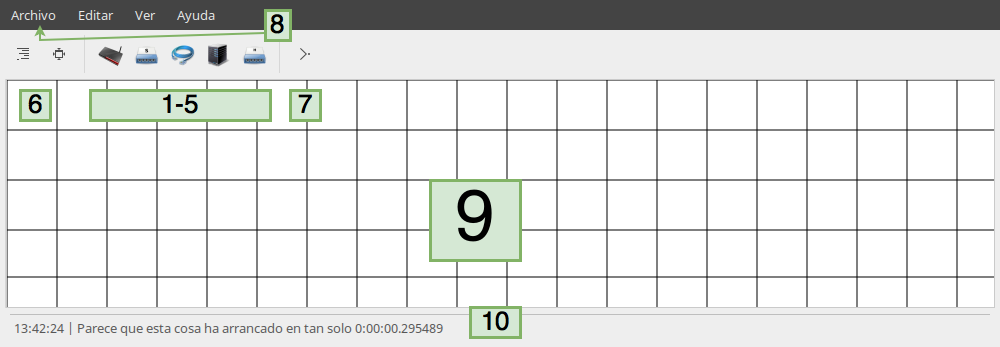
\includegraphics[width=\textwidth]{Resources/Screenshots/2016-09-07-134612_1000x700_scrot.png}
\caption[Interfaz de InvProy Alpha]{Interfaz de InvProy Alpha. Al usar Gtk+, los temas se pueden cambiar, así que la apariencia del programa puede ser distinta dependiendo del tema de escritorio que estés usando.}
\end{figure}
\newenvironment{mydescr}
{ \begin{enumerate}
    \setlength{\itemsep}{0pt}
    \setlength{\parskip}{0pt}
    \setlength{\parsep}{0pt}     }
{ \end{enumerate}                  } 
\begin{mydescr}
\item [1-5.] También se puede activar con las letras Q, W, E, R, T; respectivamente. Los botones, te permiten (de izquierda a derecha): colocar un router, colocar un switch, conectar dos objetos, colocar un ordenador y colocar un hub. Para ello primero haces click en el botón y luego haces click en el lugar donde quieras colocar el objeto. En el caso de los cables debes hacer dos clicks, uno en cada objeto a conectar. 
\item [6.] Abre el menú de ``Información de dispositivos", que proporciona información como la dirección IP y MAC, el nombre, o los dispositivos a los que está conectado. (Ver figura \ref{dispinfo}
\item [7.] Te permite enviar un ping de un ordenador a otro (El botón funciona a partir de v0.3).
\item [8.] Abre el menú de archivo, en el que puedes cargar un archivo, crear uno nuevo, guardarlo, y cerrar el programa.
\item [9.] Es la ventana donde puedes colocar los objetos. Puedes moverte a través de ella y en el menú de `Ver' puedes cambiar el que se vea la rejilla de fondo.
\item [10.] Aquí se encuentra una barra con información sobre el funcionamiento actual del programa.
\end{mydescr}
\begin{figure}[H]
\centering
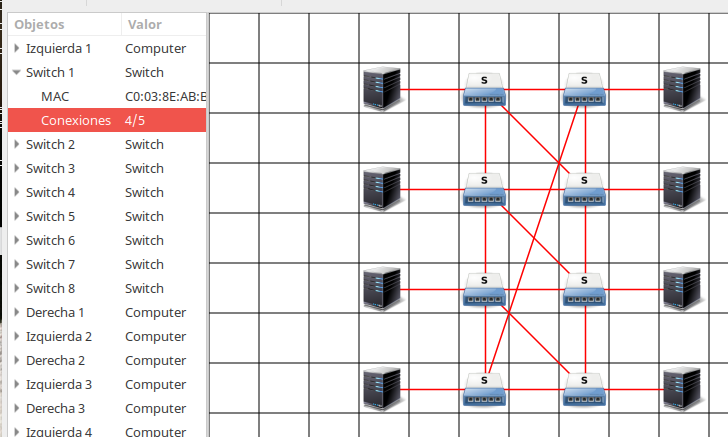
\includegraphics[width=0.9\textwidth]{Resources/Screenshots/2016-09-07-140130_728x437_scrot.png}
\caption{Menú de \textbf{Información de Dispositivos} junto a una red de topología de malla \label{dispinfo}}
\end{figure}

Para incluir un objeto en la rejilla, se hace click en el icono del objeto y luego  en el lugar donde se quiera poner. Cuando tenemos dos objetos podemos conectarlos si hacemos click primero en el icono del cable, luego en un objeto y después en otro.

Para poder enviar un paquete entre dos Computadores, necesitaremos que estén conectados mediante nodos (Hubs o Switches).

\subsection{Configuración}
Al no haber una ventana de configuración del programa, la configuración debe hacerse de forma manual editando el archivo \texttt{Config.ini} (Ver \ref{Config.ini}). Este es un archivo de texto sin formato en el que se le asigna un valor a cada variable.

\begin{easylist}[itemize]
\ListProperties(Style*=, Space*=-5pt, Space=0pt)
& \texttt{wres} y \texttt{hres}: El tamaño (en píxeles) del ancho y el alto de la ventana principal.
& \texttt{viewport-sqres}: El tamaño en píxeles del lado de los cuadrados de la rejilla.
& \texttt{viewport-wres} y \texttt{viewport-hres}: El número de cuadrados que tendrá de alto y de ancho la rejilla.
& \texttt{cable-color}: Color por defecto de los cables en HTML.
& \texttt{start-centered}: Al iniciar el programa, iniciar en el centro de la rejilla en lugar de arriba a la izquierda.
& \texttt{revealer-show-default}: (True o False). Mostrar por defecto la ventana con la información sobre los dispositivos.
& \texttt{respack}: Directorio del ``Pack de recursos"
& \texttt{routing-ttl}: Tiempo de vida en segundos de las entradas en la tabla de redireccionamiento de los switches.
& \texttt{def-max-connections}: Conexiones máximas por defecto de un conmutador/concentrador.
\end{easylist}

\section{Funcionamiento del programa}
Un programa funciona haciendo uso de todas las herramientas anteriormente mencionadas.

El programa está basado en distintas clases. Se pueden diferenciar en cuatro tipos: Clases de Interfaz (\class{MainClase}, \class{w\char`_changethings}...), 
Clases de Dispositivos (\class{ObjetoBase, Switch, Computador}), Clases de Red (\class{packet}, \class{frame}) y clases de apoyo (\class{MAC}, \class{IP}, \class{Port}, \class{Cable}).

Todas las clases poseen, como mínimo, una función llamada \function{\char`_\char`_init\char`_\char`_}, que es la encargada de crear el objeto y establecer las variables más importantes (Coordenadas, variables vacías, dirección MAC...).

\subsection{Main.py}
Es el archivo principal del programa. Contiene las funciones más importantes, además de las clases con los objetos. Primero trata de importar los módulos necesarios, comprobando uno a uno si están instalados, y advirtiendo al usuario en el caso de que no estén instalados. Podemos encontrar bastantes partes curiosas como la función \function{on\char`_key\char`_press\char`_event} de la clase \class{MainClase}, que se encarga de hacer distintas funciones cuando el usuario pulsa las distintas teclas.

\subsubsection{ObjetoBase}
En Python, existe la herencia de clases. Esto quiere decir que una clase puede heredar las funciones y los atributos de otra, en forma de cascada. La clase principal de la que heredan el resto de dispositivos de red, es esta, \class{ObjetoBase}. Algunas de sus funciones son estas:

\newpage

\begin{itemize}
\item \function{compcon}: Es una función que poseen todos los dispositivos de red, que dado un objeto \class{Computador}, retorna todos los ordenadores que están conectados a la misma red. Se encuentra en \texttt{822:864@Main.py\footnote{Notación para describir ubicación del código. Línea inicial:Línea final@Archivo. Si se omite el nombre de archivo, es el anteriormente mencionado.}}. Está formada por una lista que contendrá los ordenadores conectados y una función llamada subcompcon (\texttt{827:847}), que comprueba las conexiones del objeto, añadiendo la conexión a la lista si es un ordenador. En el caso de que sea un conmutador o un concentrador, llama a la función \texttt{subcompcon} con ese objeto como argumento, por lo que comprueba las conexiones de ese objeto y las añade a la lista del primero, entrando en un bucle hasta que ha comprobado toda la red. La función es usada por el programa cuando es necesario comprobar si dos ordenadores están conectados, por ejemplo.
\item \function{load}: \texttt{877:896} Al cargar un objeto de un archivo, hay determinadas propiedades del objeto que deben ser establecidas de cero, y determinadas funciones que deben accionarse, para ello existe esta función.
\item \function{update}: Esta función, bastante importante se encarga de actualizar la información del objeto en la interfaz de usuario. Es llamada cada vez que se produce un cambio en el objeto; como al conectarlo, editar el nombre, o desconectarlo de otros objetos.
\item \function{connect}: \texttt{898:941} Esta función se encarga de establecer las conexiones entre dos objetos.
\item \function{disconnect}: \texttt{942:989}. Realiza lo contrario de \function{connect}, desconecta un objeto de otro. O un objeto de todos a los que está conectado.
\item \function{packet\char`_received}: Esta es la función por defecto que se ejecuta cuando un dispositivo ha recibido un paquete. Todos los dispositivos de red tienen una función diferente que sobreescribe a esta (pues no es el mismo comportamiento el de un conmutador que el de un ordenador).
\end{itemize}

\begin{figure}[H]
\noindent\centering
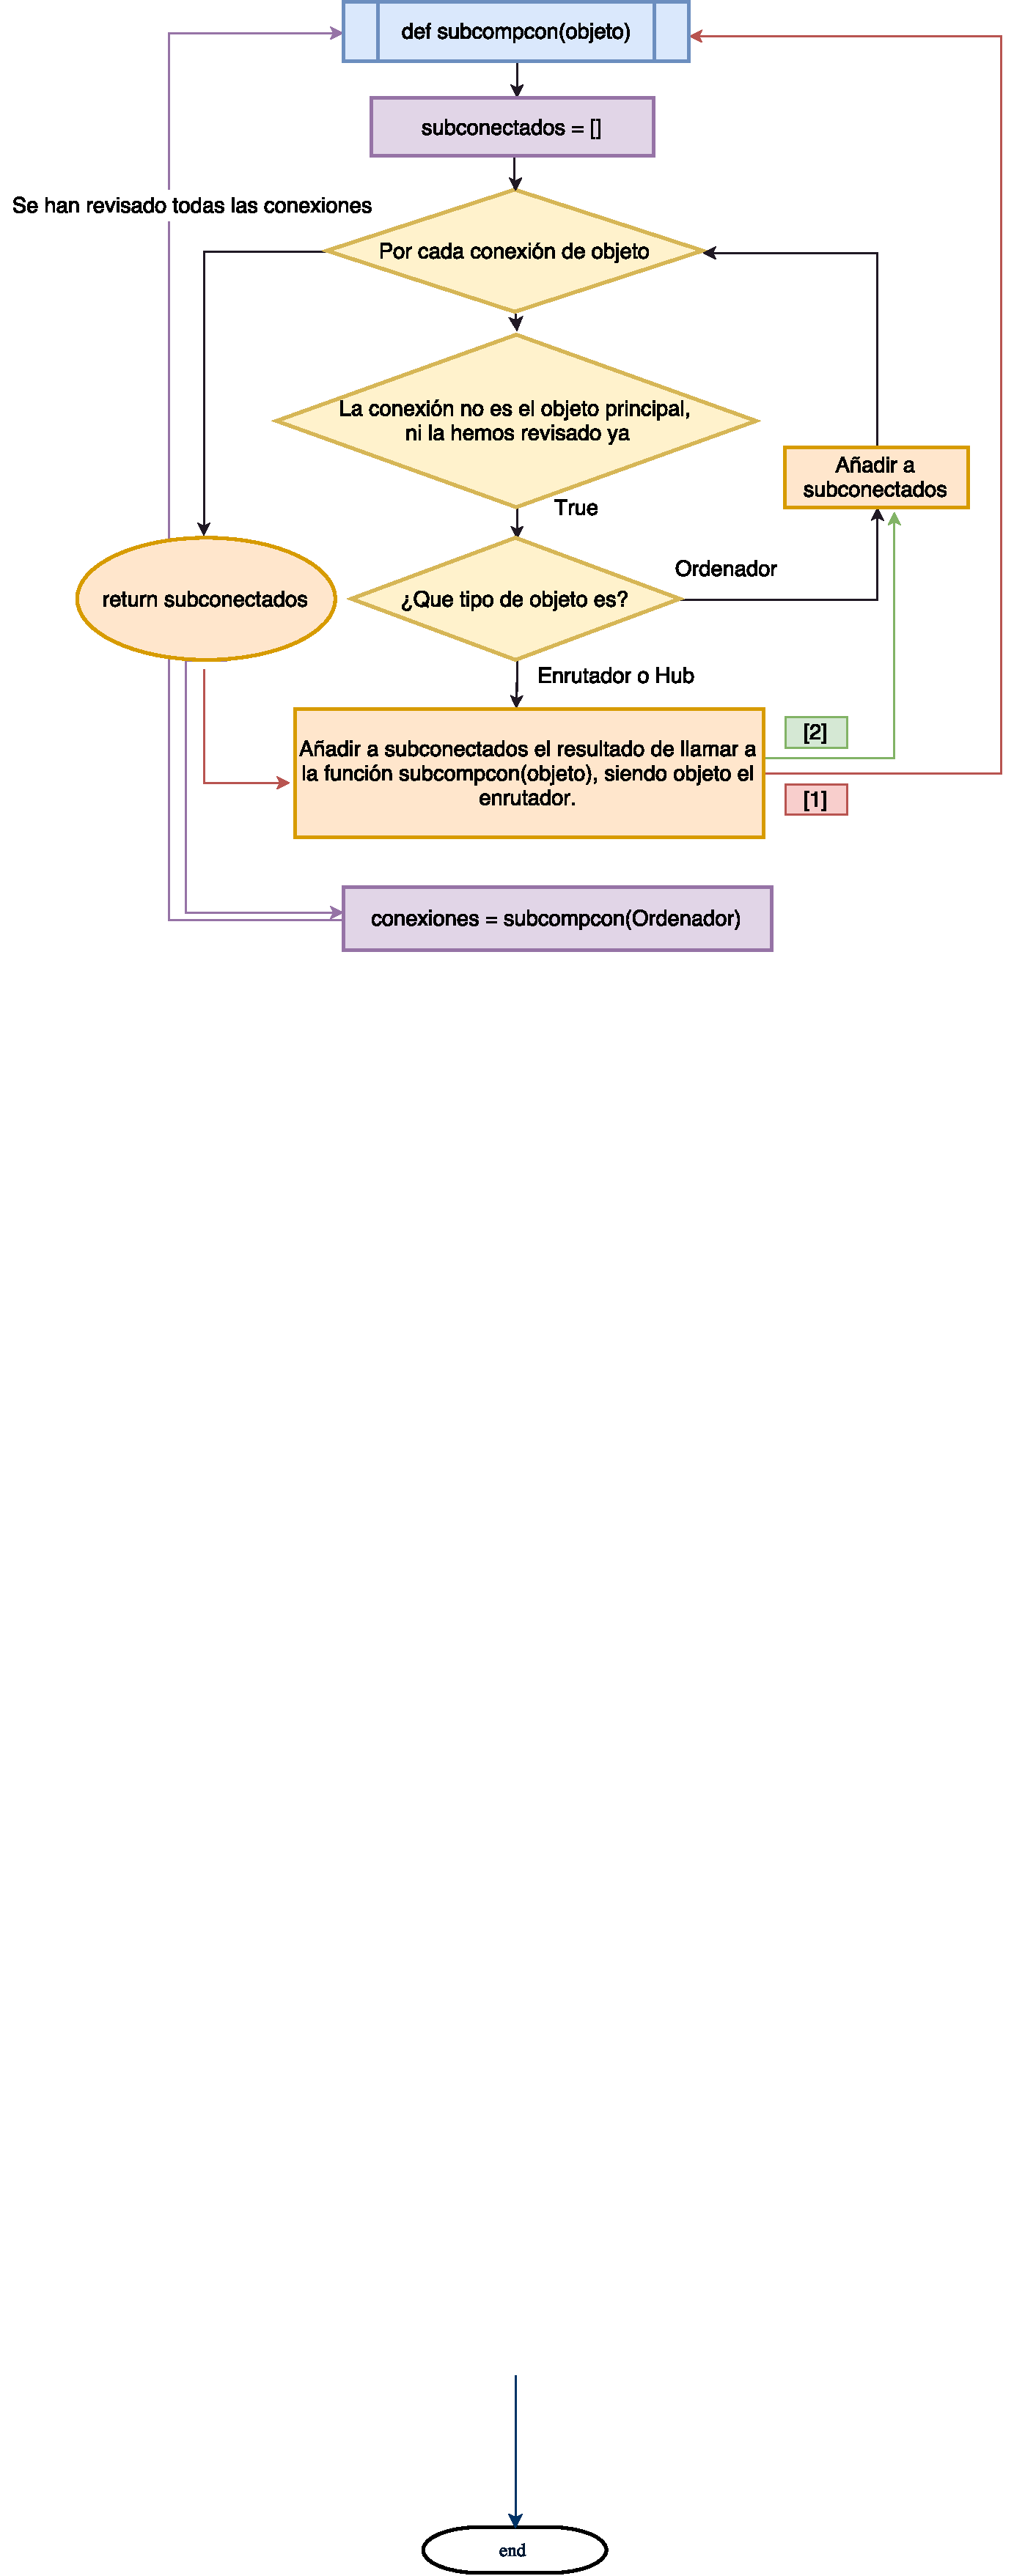
\includegraphics[width=\textwidth]{Resources/Diagramas/Compcon}
\caption[Diagrama de flujo de la función compcon]{Diagrama de flujo de la función compcon. Entra en un bucle al volver a llamar a la función de forma recursiva.}
\end{figure}

\subsubsection{mac}
Esta clase es la que crea los objetos que serán una dirección MAC. Transcurre de la línea 1024 a la 1059 y contiene varias funciones técnicas, pero la única importante es \function{genmac}, encargada de generar una dirección MAC aleatoria de 48 bits de longitud.
\subsubsection{Port y w\char`_switch\char`_table}
\class{Port} es una clase que usan los conmutadores y concentradores. Simula un puerto de red. Tan sólo posee cuatro funciones: \function{\char`_\char`_init\char`_\char`_}, que es la que se usa al crear el objeto; \function{connect}, para conectar un objeto al puerto; \function{disconnect}, para desconectarlo y \function{is\char`_available}, para saber si el puerto está disponible u ocupado. \texttt{1080:1099}

La clase \class{w\char`_switch\char`_table} es la encargada de la ventana de visualización de la tabla de enrutamiento del Switch. \texttt{1101:1160}

\subsubsection{Clases de paquetes de red}
Ocupan entre el 25\% y el 30\% del código. Son clases como \class{packet} (la clase base), \class{eth} (paquete con \textit{frame} aplicado, \class{icmp} (paquete con ICMP) y la última clase \class{Ping}, que hereda de \class{icmp} y se encarga de crear un paquete de red, bit a bit, dados una dirección IP de destino y de origen.
Entre todas estas clases debemos destacar dos funciones:
\begin{itemize}
\item \function{animate} es una función que poseen todos los tipos de paquetes de red y se encarga de poner un paquete de red en la interfaz, y de que este se mueva. Para ello, hace una combinación de dos movimientos, uno en el eje x y otro en el eje y, la longitud que debe de moverse en total la divide entre el número total de fotogramas y así consigue la distancia que debe moverse cada fotograma. Cuenta dentro con una subfunción, \function{iteration}, que se encarga de poner la imagen cada fotograma en su sitio y eliminar la imagen del fotograma anterior. Esta función ha sido posible gracias a los conocimientos adquiridos durante primero de Bachillerato.\texttt{1627:1717}
\item \function{create} es una función propiedad de \class{Ping}, dadas una dirección IP de destino y origen, crea un paquete de red, bit a bit, basado en el modelo real de paquetes de Ping inspeccionado por Wireshark, y confirmado en libros de teoría. Es una función que, aunque parezca sencilla, fueron bastantes horas de trabajo, pues es bastante complejo tratar con bits.
\end{itemize}

\subsection{save.py}
Es un archivo que se encarga de guardar y cargar archivos. Está compuesto por dos funciones: \texttt{save} y \texttt{load}, encargadas de guardar a un archivo y cargar a un archivo, respectivamente. Para ello, usan una librería nativa de Python llamada \texttt{pickle}, que se encarga de la \gls{serializar} de los objetos, y la posterior deserialización de estos. Este método de serialización debería ser cambiado en una versión posterior, ya que no es retrocompatible, es decir, no te permite cargar archivos creados con una versión anterior del programa.

\subsection{Interface.glade}
Este archivo, de otras dos mil líneas, es el encargado de establecer las propiedades de la interfaz. No ha podido ser incluido en el anexo debido a su larga extensión, ya que usa XML, un lenguaje que es bastante redundante, aunque sencillo de usar.

\subsection{Dispositivos}
Existen cuatro tipos dispositivos: los Computadores, que tienen la mayor programación; los Switches, que se encargan de manejar los paquetes de red; los Hubs, que son como los Switches, pero reenvían los paquetes por todos sus puertos y los Routers, que tan sólo existen de forma visual, pero no tienen ninguna función de momento. Por lo que sólo vamos a hablar de los Switches y los Ordenadores. Para cambiar los parámetros hay que hacer click derecho en el dispositivo al que se le deseen cambiar los parámetros y luego en la entrada de `Editar objeto'. A lo que aparecerá una ventana como la de Fig. \ref{fig:editwindow} en la que se podrán cambiar parámetros como el nombre, la dirección MAC o la dirección IP.

Los ordenadores tienen una función especial que es la de crear y enviar los paquetes de red. Para ello, en el menú emergente que aparece al hacer click derecho en el objeto, hacemos click en la entrada de `Ping'. Para que el paquete llegue al otro computador, ambos deben tener una dirección IP, y estar conectados a la misma red. Se introduce la dirección IP del dispositivo y se pulsa en el botón de `Ping!' (Ver Fig. \ref{fig:pingwindow} y Fig. \ref{fig:pingwindow2}). A continuación veremos el paquete de red buscando su objetivo, la primera vez no irá directamente, ya que los Switches están aún aprendiendo el camino, pero el paquete de vuelta y todos los siguientes paquetes seguirán la misma ruta (Ver Fig. \ref{fig:samplenet}). El ordenador crea un paquete de red usando los protocolos de Ethernet (IEEE 802.11), TCP, IPv4 e ICMP. Aquí la parte del código que, dadas dos direcciones IP's crea el binario de un Ping.

\inputminted[firstline=1782, lastline=1818, baselinestretch=1, fontsize=\scriptsize, linenos, breaklines]{python}{Codigo/Main.py}

Los Switches se encargan de redireccionar los paquetes de red. La primera vez que les llega un paquete, al no saber la ubicación física del destino, siguen este algoritmo:
\inputminted[firstline=1268, lastline=1296,baselinestretch=1,
	fontsize=\scriptsize,
	linenos,
	breaklines]{python}{Codigo/Main.py}
Este algoritmo esta basado en el que usan los conmutadores reales y, traducido a lenguaje mortal, vendría a ser:
\begin{easylist}[itemize]
\ListProperties(Style*=,Space*=6pt)
& Si la dirección MAC de destino del paquete recibido se encuentra directamente conectado al Switch y el TTL del paquete es mayor que cero:
&& Enviar el paquete a ese dispositivo.
& Al no cumplirse la condición anterior, si el paquete se encuentra en mi tabla de enrutamiento y el TTL del paquete es mayor que cero:
&& Enviamos el paquete por el puerto al que está asignada la dirección MAC en la tabla.
& Al no cumplirse las condiciones anteriores, si hay un Switch en mis conexiones y el TTL del paquete es mayor a 0:
&& Enviar el paquete a uno de los Switches de forma aleatoria.
\end{easylist}

Cuando recibe un paquete, también añade a la \textit{Routing Table} o tabla de enrutación una entrada con la dirección MAC del remitente del paquete y el puerto por el que ha llegado, así cuando le llegue un paquete el router conocerá el puerto por el que enviarlo.
\inputminted[firstline=1231, lastline=1247, baselinestretch=1,fontsize=\scriptsize, linenos,breaklines]{python}{Codigo/Main.py}
Este es el código que cumple esta función. Cada elemento en la tabla tiene un tiempo establecido en el que caduca la entrada. Lo que hace esta parte del código es comprobar si este tiempo ha caducado, actualizar la fecha de caducidad si la dirección MAC ya está en la tabla o añadirlo de nuevo en la tabla si la dirección no está.

\subsection{Ejemplo: Envío de Ping entre dos dispositivos}
Lo primero que vamos a hacer, es colocar un Switch al que poder conectar los ordenadores. Después colocamos y conectamos hasta 5 ordenadores (es el máximo de conexiones por defecto) al Switch. Después, para cada ordenador, hacemos click derecho y en el menú emergente pulsamos ``Editar Objeto", con lo que se abrirá una ventana como la de la Figura \ref{fig:editwindow}. Aquí podemos asignar una dirección IP al ordenador. Tras asignar 5 direcciones IP diferentes a los ordenadores, en cualquiera de ellos hacemos click derecho y clickamos en ``Ping", haciendo que aparezca una ventana con un cuadro de texto como en Fig. \ref{fig:pingwindow2}. En este cuadro introducimos la dirección IP del dispositivo al que queremos enviar el Ping y pulsamos la tecla Intro, así el ordenador enviará un paquete Ping Request a la IP especificada. Cuando el paquete llega al equipo con esa dirección IP, este responderá con un paquete parecido, pero en este caso será un ping de respuesta (simbolizado en rojo), por lo que el destino será el primer ordenador. En el caso de que se produzcan cambios en la red mientras el paquete viaja por esta, el paquete dispone de un tiempo de vida, por lo que cuando llega a 0 se destruye.

\section{Versión actual del programa (0.2.3-alpha)}
\label{01}
En la versión 0.1 se introdujo toda la interfaz, las conexiones, los dispositivos... Pero aún no se podían enviar ni recibir paquetes de red. En la versión 0.2 se introdujo esta posibilidad, junto a otras cosas como el enrutamiento de paquetes. El programa es considerado una versión \textit{alpha}, ya que aún está en desarrollo y no es un programa terminado.

El programa te permite, por el momento, hacer una simulación de red simple. Se podría decir que es una base sobre la que se pueden ir añadiendo más funcionalidades, como el soporte para otros protocolos, o un modo `explicatorio' que enseñe a los alumnos lo que está pasando en la red. En la versión 0.2.3-alpha del programa sólo se ha introducido el ``Ping", es decir, la posibilidad de enviar un paquete de prueba a otro dispositivo de la misma red. También se han introducido algunos cambios en la interfaz, uno de ellos, bastante útil para el aprendizaje: los cuadros de texto en los que se introducen direcciones IP, cambian de color entre rojo, naranja o verde, dependiendo si la IP introducida no es válida, está incompleta o es válida, respectivamente.

\section{Desarrollo del proyecto}
En cuanto al código, a pesar de la gran extensión del programa, han sido escritas muchas más líneas, que han sido en algún momento eliminadas o reemplazadas. El desarrollo del proyecto puede dividirse en 4 fase, una por trimestre, aproximadamente.

En la primera fase, de Noviembre a Febrero/Marzo he ido aprendiendo sobre todo de Gtk+, la librería para la interfaz del programa. Al empezar el proyecto mis conocimientos sobre esta librería eran nulos; y sobre Python, el lenguaje de programación, eran demasiado básicos. También aprendí bastante sobre redes informáticas.

En la segunda fase, se fue desarrollando la ``base" del programa, transcurre de Febrero-Marzo a finales de curso. La interfaz, las ideas, las conexiones de los cables... Se construye la versión 0.1, como menciono en \ref{01}. El programa contaba con unas 700 líneas en \texttt{Main.py}

En la tercera fase se desarrolla la gran parte del programa, aquí es cuando llega a las 2000 líneas, sin mencionar los pequeños módulos y otros archivos. Transcurre en verano, entre Junio y mediados de Agosto. Con una media de 200-300 líneas semanales y picos de hasta mil líneas entre el 7 y el 14 de Agosto, ha sido posible cumplir el objetivo de crear un pequeño simulador de redes. Es el desarrollo de la versión 0.2-alpha, ya que el programa sigue en desarrollo de posteriores versiones.

La cuarta fase transcurre solapada con la tercera, comienza en Julio y acaba el día \@date, con la entrega de la memoria del proyecto. Es la fase en la que se desarrolla esta memoria.

He notado bastante la adquisición de experiencia, ya que tardé prácticamente 5-6 meses en hacer las primeras 500 líneas; pero en verano, conforme iba programando más, conseguí llegar a hacer más de 1000 líneas en una semana.

\subsection{Obstaculos en el desarrollo del proyecto}
Durante el desarrollo del proyecto han surgido bastantes trabas y contratiempos, que he conseguido solucionar. Muchos de ellos surgen por la falta del gran conocimiento técnico necesario para la creación de un software tan específico, han sido muchas horas de mirar la documentación de las librerías \cite{PyGiApi}, y pedir ayuda por foros para intentar solucionar dudas y bugs.

En algunas ocasiones no han sido errores, sino falta de conocimiento para el desarrollo de determinadas funciones lo que ha creado pausas de hasta dos semanas en la acción de escribir el programa.

\section{Conclusión}
Lo más difícil fue empezar. El tratar de aprender tanta información de golpe de forma autodidacta... Aunque ya supiese un poco sobre programación en Python, no tenía casi experiencia, aprender a usar la librería de Gtk+, aprender sobre redes, aprender sobre un uso más extenso de GNU/Linux, aprender sobre \LaTeX , etc. fue bastante cansado. pero eso es lo mejor, todo lo que he aprendido y, sobre todo, la experiencia que he adquirido en el campo de la programación.

A la hora de programar, al principio el ritmo era muy lento, de unas 200 líneas al mes, con pausas de semanas para solucionar problemas y errores. Poco a poco se fue acelerando hasta llegar a finales de Julio, donde hacía más de 100 líneas diarias.

Pese a que es verdad que falta incluir más protocolos y algunas funcionalidades bastante básicas (como mover objetos), estoy bastante satisfecho con la versión actual del programa, que se ha realizado con bastante poco tiempo, ya que tiene las bases, y creo que añadir un nuevo protocolo, o una nueva funcionalidad no serían más que unas horas delante de la pantalla y el teclado del ordenador.

\glsaddall
\renewcommand{\glsnamefont}[1]{\makefirstuc{#1}}
\renewglossarystyle{mcolindex}{%
  \setglossarystyle{index}%
  \renewenvironment{theglossary}%
    {%
     \begin{multicols}{\glsmcols}
     \setlength{\parindent}{0pt}%
     \setlength{\parskip}{0pt plus 0.3pt}%
     \renewcommand\item{\par\hangindent7pt}}%
    {\end{multicols}}%
}

\nocite{*}
%\bibliographystyle{IEEEtranN}
\printbibliography[heading=bibintoc]

\appendix
\printglossary[type=\acronymtype, style=mcolindex, title=Glosario y acrónimos, toctitle=Glosario y acrónimos]

\chapter{Unidades de transferencia de datos}
{\setstretch{1.3}
Cantidad de datos transferidos por unidad de tiempo. La unidad de tiempo es el segundo y la cantidad de datos puede ser medida en \textit{\glspl{bit}} (bitrate), carácteres/símbolos (\textit{baudrate}) o bytes (8 bits), en ocasiones también se utilizan \textit{nibbles} (4 bits). Para expresar esta velocidad, se suelen usar múltiplos, que pueden ser en base binaria (Sistema del IEEE) o decimal (Sistema Internacional).

Se usa la ``b" para designar los bits, y ``B" para los Bytes. Después, se usan los prefijos del sistema internacional cuando es en base decimal, y los prefijos del SI cambiando la segunda sílaba por ``bi" (e.g: kilobit / kibibit, kbit/s / Kibit/s) cuando se trata de múltiplos binarios.
}
\newcolumntype{R}{>{\raggedleft\arraybackslash}X}
\section*{Tabla de múltiplos}
\noindent
\begin{tabularx}{\columnwidth}{| l >{\centering}X X|}
\rowcolor{header} \hline
\textbf{Unidad} & \textbf{Símbolo} & \textbf{Equivalencia} \\ \hline
Kilobit/s & kbit/s o kb/s & 1000 bit/s \\
Megabit/s & Mbit/s o Mb/s & $\mathsf{10^{6}}$ bit/s o 10³ kbit/s  \\
Gigabit/s & Gbit/s o Gb/s & $\mathsf{10^{9}}$ bit/s o 10³ Mb/s \\
Terabit/s & Tbit/s o TB/s & $\mathsf{10^{12}}$ bit/s o 10³ Gb/s \\ \hline
Kibibit/s & Kibit/s & $\mathsf{2^{10}}$ bit/s o 1024 bit/s \\
Mebibit/s & Mibit/s & $\mathsf{2^{20}}$ bit/s o 1024 Kibit/s \\
Gibibit/s & Gibit/s & $\mathsf{2^{30}}$ bit/s o 1024 Mibit/s \\
Tebibit/s & Tibit/s & $\mathsf{2^{40}}$ bit/s o 1024 Gibit/s \\ \hline \hline
Byte/s    & Byte/s & 8 bit/s \\
Kilobyte/s & kB/s & 1000 Byte/s o 8000 bits/s \\
Megabyte/s & MB/s & $\mathsf{10^{6}}$ Byte/s o 1000 kB/s \\
Gigabyte/s & GB/s & $\mathsf{10^{9}}$ Byte/s o 1000 MB/s \\
Terabyte/s & TB/s & $\mathsf{10^{12}}$ Byte/s o 1000 GB/s \\ \hline
Kibibyte/s & KiB/s & 1024 Byte/s \\
Mebibyte/s & MiB/s & $\mathsf{2^{20}}$ Byte/s \\
Gibibyte/s & GiB/s & $\mathsf{2^{30}}$ Byte/s \\
Tebibyte/s & TiB/s & $\mathsf{2^{40}}$ Byte/s \\ \hline
\end{tabularx}

\chapter{Capturas de pantalla del programa}
\noindent\begin{figure}[H]
\centering
\begin{minipage}[t]{0.4\textwidth}
	%\vtop{
	\centering
	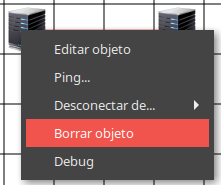
\includegraphics[scale=0.6]{Resources/Screenshots/2016-09-12-172627_1000x700_scrot.png}%}
	\caption{Captura: Click derecho en un computador}
\end{minipage}
\hspace*{0.15\textwidth}
\begin{minipage}[t]{0.4\textwidth}
	%\vtop{
	\centering
	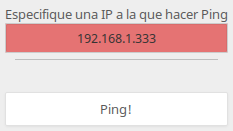
\includegraphics[width=\textwidth]{Resources/Screenshots/2016-09-12-225752_233x131_scrot.png}%}
	\caption[Captura: Ventana para enviar ping.]{Captura: Ventana para enviar ping. Está en rojo porque la IP introducida no es válida.}
	\label{fig:pingwindow}
\end{minipage}

\centering
\begin{minipage}[t]{0.4\textwidth}
	\centering
	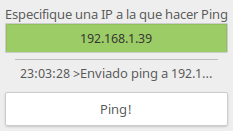
\includegraphics[width=\textwidth]{Resources/Screenshots/2016-09-12-230329_233x131_scrot.png}
	\caption{Captura: Igual que \ref{fig:pingwindow}, pero con una IP válida.}
	\label{fig:pingwindow2}
\end{minipage}
\hspace*{0.15\textwidth}
\begin{minipage}[t]{0.4\textwidth}
	\centering
	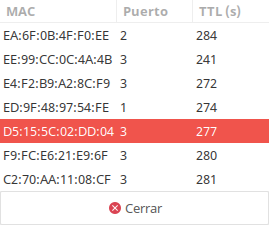
\includegraphics[scale=0.6]{Resources/Screenshots/2016-09-12-230428_269x225_scrot.png}
	\caption{Captura: Ventana con la tabla que poseé el Switch.}
	\label{fig:switchingtable}
\end{minipage}

\centering
\begin{minipage}[t]{0.5\textwidth}
	\centering
	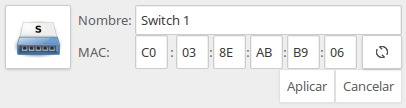
\includegraphics[scale=0.6]{Resources/Screenshots/2016-09-13-200254_406x108_scrot.png}
	\caption{Captura: Ventana de edición de propiedades de objeto.}
	\label{fig:editwindow}
\end{minipage}

\end{figure}
\begin{figure}[H]
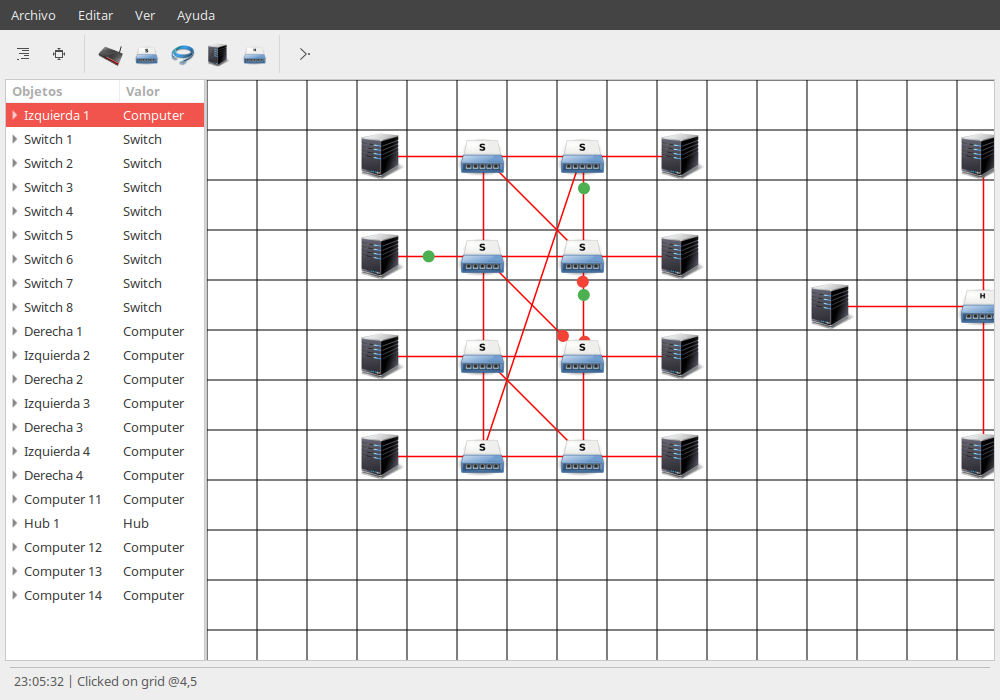
\includegraphics[width=\textwidth]{Resources/Screenshots/2016-09-12-230644_1000x700_scrot.png}
\caption{Captura: Paquetes viajando por una red de ejemplo.}
\label{fig:samplenet}
\end{figure}

\chapter[Licencia GNU GPL]{Licencia GNU General Public License}
\label{gnugpl}
Es la licencia más usada en el desarrollo de software. Permite las cuatro libertades del software libre y fue creada por la Free Software Foundation. La versión más reciente, la GPLv3, ha sido publicada el 29 de junio de 2007. Al distribuir el programa, debe distribuirse también una copia de la licencia que usa. 

InvProy usa la licencia GPLv3, aquí una traducción no oficial\cite{gpltranslation}:
\inputminted[baselinestretch=1, fontsize=\scriptsize, linenos, breaklines]{text}{GPLv3-spanish.txt}

\chapter{Código del programa}
%\begin{listing}
\newcommand{\ipm}[1]{
	\section{#1}
	\inputminted[baselinestretch=1, fontsize=\tiny, linenos, breaklines]{python}{Codigo/#1}
}
\ipm{Main.py}
\ipm{Modules/logmod.py}
\ipm{Modules/save.py}
%\section{Interface2.glade} \inputminted[baselinestretch=1, fontsize=\scriptsize, linenos, breaklines]{XML}{Codigo/Interface2.glade}

%\end{listing}

\newpage
\thispagestyle{empty}
\topskip0pt
\vspace*{\fill}
\doclicenseThis
\vspace*{\fill}
\end{document}
